\documentclass[a4paper,12pt]{report}

% Page layout
\usepackage[left=2.5cm,right=2.5cm,top=2.5cm,bottom=2.5cm]{geometry}

% Font and text
\usepackage[english]{babel}
\usepackage{microtype}
\usepackage{setspace}
\usepackage{lmodern}
\usepackage{siunitx}
\newcommand{\myemph}[1]{{\sffamily\bfseries#1}}
\sloppy
\onehalfspacing

% Headings
\usepackage[raggedright,sf,bf]{titlesec}
\usepackage[margin=\the\parindent,small,bf,sf]{caption}
\titlelabel{\thetitle.\ }
\titleformat{\chapter}[display]{\huge\bfseries\sffamily}{\chaptertitlename\ \thechapter}{15pt}{\Huge \raggedright}
\titlespacing*{\chapter}{0pt}{0pt}{40pt}  % remove spacing before chapter headings
\makeatletter
\let\originall@chapter\l@chapter
\def\l@chapter#1#2{\originall@chapter{{\sffamily #1}}{#2}}
\makeatother

%% Alternative headings using small-caps (comment out the top section)
%\usepackage[raggedright,bf]{titlesec}
%\usepackage[margin=\the\parindent,small,bf]{caption}
%\titlelabel{\thetitle.\ }
%\titleformat{\chapter}[display]{\huge\scshape}{\chaptertitlename\ \thechapter}{15pt}{\Huge \raggedright}
%\titlespacing*{\chapter}{0pt}{0pt}{40pt}  % remove spacing before chapter headings

% Table of contents
\let \savenumberline \numberline
\def \numberline#1{\savenumberline{#1.}}

% Figures
\usepackage{graphicx}
\usepackage{pdfpages}
\usepackage{subcaption}
\setlength{\abovecaptionskip}{7.5pt}  % spacing above and below captions
\newcommand*{\WaterMark}[2][0.2\paperwidth]{\AddToShipoutPicture*{\AtTextCenter{\parbox[c]{0pt}{\makebox[0pt][c]{\includegraphics[width=#1]{#2}}}}}}

% Mathematics
\usepackage[cmex10]{amsmath}
\usepackage{amssymb}
\usepackage{cancel}
\DeclareMathOperator*{\argmax}{arg\,max}
\newcommand{\T}{^\top}
\newcommand{\tr}{\textrm{tr}}
\renewcommand{\vec}[1]{\boldsymbol{\mathbf{#1}}}
\newcommand{\defeq}{\triangleq}

% Tables
\usepackage{booktabs}
\usepackage{tabularx}
\usepackage{multirow}
\newcommand{\mytable}{
    \centering
    \small
    \renewcommand{\arraystretch}{1.2}
    }
\renewcommand{\tabularxcolumn}[1]{m{#1}}
\newcolumntype{C}{>{\centering\arraybackslash}X}
\newcolumntype{L}{>{\raggedright\arraybackslash}X}

% Header and footer
\usepackage{fancyhdr}
\pagestyle{fancy}
\fancyhf{}
\renewcommand{\sectionmark}[1]{\markright{\normalsize \thesection.\ #1}}
\fancyhead[C]{\nouppercase{\textit{\rightmark}}}
\fancyhead[RO]{\thepage}
 \fancyhead[LE]{\thepage}  % double-sided printing
\fancyfoot{}
\setlength\headheight{14.5pt}
\renewcommand{\headrulewidth}{0pt}
\fancypagestyle{plain}{\fancyhead{}
                       \renewcommand{\headrulewidth}{0pt}
                       \fancyfoot[C]{\thepage}}

% Pseudo-code
\usepackage{algorithm}  % should go before \usepackage{hyperref}

% Table of contents and hyperlinks
\usepackage{hyperref}
\hypersetup{colorlinks=true,linktoc=all,citecolor=black,linkcolor=black}
\usepackage[nottoc]{tocbibind}

% Pseudo-code
\usepackage{algpseudocode}  % should go after \usepackage{hyperref}
\renewcommand{\thealgorithm}{\arabic{chapter}.\arabic{algorithm}} 
\captionsetup[algorithm]{labelfont={bf,sf},font=small,labelsep=colon}

% Bibliography
\usepackage{cite}  % automatically reorder inline citations
\bibliographystyle{IEEEtran}

% Fix titlesec issue
\usepackage{etoolbox}
\makeatletter
\patchcmd{\ttlh@hang}{\parindent\z@}{\parindent\z@\leavevmode}{}{}
\patchcmd{\ttlh@hang}{\noindent}{}{}{}



\makeatother


\begin{document}

% Front matter
\graphicspath{{frontmatter/fig/}}
\pagenumbering{Alph}

\begin{titlepage}
	\begin{center}
		
		
\includegraphics[width=10cm]{US}
		
		\vfill
		
		{\sffamily \bfseries \huge Development of a tool for the extraction of low frequency mean square flux noise figures in SQUIDs \par}
%		{\scshape \huge A Critical Analysis of Design Flaws in the Death Star \par}
		
		\vfill
		
		{\large {\Large Paul Rossouw} \\ 23572027 \par}
		
		\vfill
		
		\vfill
		
		{Report submitted in partial fulfilment of the requirements of the module \\
			Project (E) 448 for the degree Baccalaureus in Engineering in the Department of
			Electrical and Electronic Engineering at Stellenbosch University. \par}
		
		\vfill
		
		{\large {Supervisor}: Prof C.\ J.\ Fourie} %\\
		% Department of Electrical and Electronic Engineering \par}
		
		\vfill
		
		{\Large October 2023}
	\end{center}
\end{titlepage}

%\graphicspath{{frontmatter/fig/}}
\pagenumbering{Alph}

\begin{titlepage}
	\begin{center}
		
		%
\includegraphics[width=10cm]{USlogo-top}
		
		\WaterMark{UScrest-WM}
		
		~\vspace{4.5em}
		
		{\sffamily \bfseries \huge A Critical Analysis of Design Flaws in the Death Star \par}
%		{\scshape \huge A Critical Analysis of Design Flaws in the Death Star \par}		
		
		\vspace{7em}
		
		{\large {\Large  Luke Skywalker} \\ 99652154 \par}
		
		\vspace{8em}
		
		{\large Thesis presented in partial fulfilment of the requirements for the degree of \\ Master of Engineering (Electronic) in the Faculty of Engineering at Stellenbosch University. \par}
		
		\vfill
		
		{\large {Supervisor}: Dr O.\ W.\ Kenobi\\
		Department of Electrical and Electronic Engineering \par}
		
		%\vfill
		\vspace{10em}
		
		{\Large October 2099}
	\end{center}
\end{titlepage}

\pagenumbering{roman}
\chapter*{Acknowledgements}
% \addcontentsline{toc}{chapter}{Acknowledgements}
\makeatletter\@mkboth{}{Acknowledgements}\makeatother

Firstly I would like to thank my parents for their unconditional love and support. They have made this journey possible. I would also like to thank my brother and sister for always challenging me. Lastly, I would like to thank my oupa Dawie for inspiring me to pursue a technical degree. 
%\chapter*{Declaration}
\newpage
\thispagestyle{plain}
\addcontentsline{toc}{chapter}{Declaration}
\makeatletter\@mkboth{}{Declaration}\makeatother

\centerline{
\includegraphics[width=8cm]{USlogo-top}}
\vspace*{-10pt}

\section*{\centering Plagiaatverklaring / \textit{Plagiarism Declaration}}

\vspace*{5pt}

\begin{enumerate}
    \item Plagiaat is die oorneem en gebruik van die idees, materiaal en ander intellektuele eiendom van ander persone asof dit jou eie werk is.\\
    \textit{Plagiarism is the use of ideas, material and other intellectual property of another's work
        and to present is as my own.}
    
    \item Ek erken dat die pleeg van plagiaat 'n strafbare oortreding is aangesien dit 'n vorm van diefstal is.\\
    \textit{I agree that plagiarism is a punishable offence because it constitutes theft.}
    
    \item Ek verstaan ook dat direkte vertalings plagiaat is. \\
    \textit{I also understand that direct translations are plagiarism.}
    
    \item Dienooreenkomstig is alle aanhalings en bydraes vanuit enige bron (ingesluit die internet) volledig verwys (erken). Ek erken dat die woordelikse aanhaal van teks sonder aanhalingstekens (selfs al word die bron volledig erken) plagiaat is. \\
    \textit{Accordingly all quotations and contributions from any source whatsoever (including the internet) have been cited fully. I understand that the reproduction of text without quotation marks (even when the source is cited) is plagiarism}
    
    \item Ek verklaar dat die werk in hierdie skryfstuk vervat, behalwe waar anders aangedui, my eie oorspronklike werk is en dat ek dit nie vantevore in die geheel of gedeeltelik ingehandig het vir bepunting in hierdie module/werkstuk of 'n ander module/werkstuk~nie. \\
    \textit{I declare that the work contained in this assignment, except where otherwise stated, is my original work and that I have not previously (in its entirety or in part) submitted it for grading in this module/assignment or another module/assignment.}
\end{enumerate}

\vfill

\noindent \begin{tabularx}{1.0\linewidth}{|L|L|}
    \hline
    \vspace{1cm} {Studentenommer / \textit{Student number}} & \vspace{1cm} {Handtekening / \textit{Signature}} \\
    \hline
    \vspace{1cm} {Voorletters en van / \textit{Initials and surname}} & \vspace{1cm} {Datum / \textit{Date}} \\
    \hline
\end{tabularx}

\vspace{15pt}

% The old declaration

%I, the undersigned, hereby declare that the work contained in this report is my own original work unless otherwise stated.
%
%% Afrikaans:
%% Hiermee verklaar ek, die ondergetekende, dat die werk in hierdie verslag vervat my eie oorspronklike werk is, tensy anders vermeld.
%
%\vspace{2.5cm}
%
%\begin{table}[h]
%\begin{tabular}{@{}p{2.5cm}p{5cm}}
%    Signature: & \dotfill \\
%    & \multicolumn{1}{c}{Obi-Wan Kenobi} \\
%    ~\vspace{1cm} \\
%    Date: & \dotfill \\
%\end{tabular}
%\end{table}
%
%\vfill
%
%\begin{center}
%    Copyright \textcopyright\ 2099 Stellenbosch University \\
%    All rights reserved
%\end{center}


\chapter*{Abstract}
\addcontentsline{toc}{chapter}{Abstract}
\makeatletter\@mkboth{}{Abstract}\makeatother

\subsubsection*{English}

The phenomenon of 1/f flux noise in superconducting quantum interference devices (SQUIDs) is known to be the limiting factor in the performance of biomagnetic sensors and qubits. In this project a numerical framework for calculating the mean square flux noise (MSFN) figure for an arbitrary SQUID design is implemented. The implementation aims to be flexible such that changes in the numerical framework does not require significant changes in the implementation. The project demonstrates how InductEx can be used for this purpose. It further describes the design and implementation of an optimisation technique. Results show that the model for the 1/f noise chosen is not correct but still has potential as a useful tool for design. The optimisation technique shows promising results and can speed up computation time by a factor of 180 while introducing a maximum error of $8\%$. Recent studies suggest more sophisticated models that are extensions of the model assumed in the derivation of the numerical framework. These models could potentially be implemented by extending the implementation presented in this project.

\selectlanguage{afrikaans}

\subsubsection*{Afrikaans}

Die verskynsel van 1/f  magnetiese vloed steurings in superconducting quantum interference devices (SQUIDs) is bekend as die beperkende faktor in die ontwikkeling van beter biomagnetiese sensore en qubits. In hierdie projek word 'n numeriese raamwerk geïmplementeer om die gemiddelde kwadraat magnetiese vloed steurings (MSFN) waarde vir 'n willekeurige SQUID-ontwerp te bereken. Die implementasie streef daarna om aanpasbaar te wees, sodat veranderinge in die numeriese raamwerk nie 'n betekenisvolle verandering in die implementasie vereis nie. Die projek demonstreer hoe InductEx vir hierdie doel gebruik kan word. Die projek beskryf verder die ontwerp en implementasie van 'n optimiserings tegniek. Die resultate toon aan dat die gekose model vir die 1/f magnetiese vloed steurings nie korrek is nie, maar steeds potensiaal het as 'n nuttige hulpmiddel vir ontwerp. Die optimiserings tegniek toon belowende resultate en kan berekeningstyd met 'n faktor van 180 versnel, met 'n maksimum fout van $8\%$. Onlangse studies suggereer meer gesofistikeerde modelle wat uitbreidings is van die model wat in die afleiding van die numeriese raamwerk aanvaar is. Hierdie modelle kan moontlik geïmplementeer word as 'n uitbreiding van die implementasie wat in hierdie projek aangebied word.

\selectlanguage{english}
\tableofcontents
\listoffigures
\listoftables
\chapter*{Nomenclature\markboth{}{Nomenclature}}
\addcontentsline{toc}{chapter}{Nomenclature}

% \vspace*{-3mm}
\subsubsection*{Variables and functions}

\begingroup
\renewcommand{\arraystretch}{1.2}
\renewcommand{\tabularxcolumn}[1]{p{#1}}
\begin{tabularx}{\textwidth}{@{}p{2.5cm}L}
    $p(x)$ & Probability density function with respect to variable $x$.\\
    $P(A)$ & Probability of event $A$ occurring.\\
    $\varepsilon$ & The Bayes error. \\
    $\varepsilon_u$ & The Bhattacharyya bound. \\
    $B$ & The Bhattacharyya distance. \\
    $s$ & An HMM state.  A subscript is used to refer to a particular state, e.g.\ $s_i$ refers to the $i^{\text{th}}$ state of an HMM. \\
    $\mathbf{S}$ & A set of HMM states. \\
    $\mathbf{F}$ & A set of frames. \\
    $\mathbf{o}_f$ & Observation (feature) vector associated with frame $f$. \\
    $\gamma_s(\mathbf{o}_f)$ & A posteriori probability of the observation vector $\mathbf{o}_f$ being generated by HMM state $s$. \\
    $\mu$ & Statistical mean vector. \\
    $\Sigma$ & Statistical covariance matrix. \\
    $L(\mathbf{S})$ & Log likelihood of the set of HMM states $\mathbf{S}$ generating the training set observation vectors assigned to the states in that set. \\
    $\mathcal{N}(\mathbf{x} | \mu, \Sigma)$ & Multivariate Gaussian PDF with mean $\mu$ and covariance matrix $\Sigma$.\\
    $a_{ij}$ & The probability of a transition from HMM state $s_i$ to state $s_j$. \\
    $N$ & Total number of frames or number of tokens, depending on the context. \\
    $D$ & Number of deletion errors. \\
    $I$ & Number of insertion errors. \\
    $S$ & Number of substitution errors. \\
\end{tabularx}
\endgroup


\newpage
\subsubsection*{Acronyms and abbreviations}

\begingroup
\renewcommand{\arraystretch}{1.2}
\begin{tabular}{@{}p{2.5cm} l}
    AE      & Afrikaans English \\
    AID     & accent identification \\
    ASR     & automatic speech recognition \\
    AST     & African Speech Technology \\
    CE      & Cape Flats English \\
    DCD     & dialect-context-dependent \\
    DNN		& deep neural network \\
    G2P     & grapheme-to-phoneme \\
    GMM     & Gaussian mixture model \\
    HMM     & hidden Markov model \\
    HTK     & Hidden Markov Model Toolkit \\
    IE      & Indian South African English \\
    IPA     & International Phonetic Alphabet \\
    LM      & language model \\
    LMS     & language model scaling factor \\
    MFCC    & Mel-frequency cepstral coefficient \\
    MLLR    & maximum likelihood linear regression \\
    OOV     & out-of-vocabulary \\
    PD      & pronunciation dictionary \\
    PDF     & probability density function \\
    SAE     & South African English \\
    SAMPA   & Speech Assessment Methods Phonetic Alphabet \\
\end{tabular}
\endgroup

\newpage
\pagenumbering{arabic}

% Contents
\graphicspath{{introduction/fig/}}

\chapter{Introduction}
\label{chap:introduction}




\graphicspath{{litreview/fig/}}

\chapter{Literature Review}
\label{chap:litreview}


\section{Theory and applications of superconductivity}
In order to understand and apply the methods described in \cite{fluxNoiseSquidsStevenAnton} one must first understand the basic theory behind superconductivity as well as some examples of how this theory is used in practice.

\subsection{Superconductivity}
\textcolor{red}{REVIEW NEEDED}

Since the first discovery of superconductivity a couple of successfully theories have been put forth to explain the phenomenon. The London theory is a framework that describes the qualitative behaviour of superconductors and correctly describes perfect diamagnetic and zero resistance but fails to explain the effect on a microscopic level \cite{Golubov_1998}. The London equations (equation \ref{london1} and equation \ref{london2}) \cite{Tinkham_2015} is an addition to Maxwell's equations.
\begin{equation}
    E = \frac{\partial}{\partial t}(\Lambda J_s)
    \label{london1}
\end{equation}
\begin{equation}
    h = -c \nabla\times (\Lambda J_s)
    \label{london2}
\end{equation}
Here $\Lambda$ is a phenomenological parameter determined through experimentation. The London equations allow us to calculate the current distribution in a superconductor which is very important to the objective of this project. BCS theory put forth a microscopic model of superconductors and explains the phenomenon as a quantum mechanical effect. The details are out of scope for this project but on a crude qualitative level BCS theory can be explained by the pairing of electrons in the crystal lattice of the superconductor allowing them to be considered one particle. These particles are known as cooper-pairs. At extremely low temperatures the formation of these cooper pairs are energetically favourable \cite{Feynman_Leighton_Sands_2013}. Electron pairs in this state can flow through the superconductor unimpeded. BCS theory is the most successful model of superconductivity discovered to date. 

\subsection{The Josephson junction}
In superconducting electronics the active component is the Josephson junction \cite{Duzer_1999_Princip_Super}. The Josephson junction refers to a situation where two superconductors are connected through a thin non-conductive barrier. If this barrier is thin enough one can observe what is known as the Josephson effect. This phenomenon is can be explained by considering the effect of quantum tunnelling of cooper pairs through the non-conductive boundary. For a sufficiently large barrier one can express the ensemble average wave function in each superconductor independently\cite{Duzer_1999_Princip_Super}:
\begin{equation}
    \Psi = |\Psi(\Vec{r})| \exp{\{i\theta(\Vec{r})\}}
    \label{eq:ensembleWave}
\end{equation}
This is due to the fact that it is energetically favourable for cooper pairs in proximity to one another to lock phases \cite{Duzer_1999_Princip_Super} allowing one to express a large collection of these cooper pairs as one ensemble wave function. The idea that it is energetically favourable for cooper-pairs in proximity to one another extends to the situation where the superconductors are separated by an insulating boundary. When the barrier is sufficiently small the energy of the system can be reduced by the coupling of wave functions in their respective superconductors \cite{Duzer_1999_Princip_Super}. This results in cooper-pairs being able to move across the boundary without energy loss. Following the derivation in \cite{Feynman_Leighton_Sands_2013} one can describe the system behaviour using Schrödinger's equation when a voltage is applied to the junction \cite{Feynman_Leighton_Sands_2013}: 
\begin{equation}
    i\hbar \frac{\partial\Psi_1}{\partial t} = U_1\Psi_1 +K\Psi_2 
    \label{eq:shrod1}
\end{equation}
\begin{equation}
    i\hbar \frac{\partial\Psi_2}{\partial t} = U_2\Psi_2 +K\Psi_1
    \label{eq:shrod2}
\end{equation}
Here $U_1 = qV/2$ and $U_2 = -qV/2$ \cite{Feynman_Leighton_Sands_2013} refer to the energy of the two wave functions and $K$ refers to the coupling energy between each wave function. By taking \ref{eq:ensembleWave} and setting $|\Psi(\Vec{r})|$ to $\sqrt{\rho}$ where $\rho$ refers to the cooper pair density in the super conductor one can substitute the result into equations \ref{eq:shrod1} and \ref{eq:shrod2}. From this substitution one can find that the rate of change of electron density on either side of the junction to be described by the following equation \cite{Feynman_Leighton_Sands_2013}:

\begin{equation}
    \dot\rho_1 = \frac{2}{\hbar}K\sqrt{\rho_1\rho_2}sin(\delta)
    \label{eq:charge_dens}
\end{equation}

Where $\rho_1$ is the electron density on one side of the junction. The rate of change of charge on the other side of the junction is simply $\dot\rho_2 = -\dot\rho_1$\cite{Feynman_Leighton_Sands_2013}. The rate of change of charge is the current and therefore the current through the junction can be expressed as follows \cite{CPRJJ}:

\begin{equation}
    I = I_0sin(\theta_2 - \theta_1)
    \label{eq:joseph}
\end{equation}

Equation \ref{eq:joseph} is known as the current-phase relation of the DC Josephson effect.
The phases of the currents on each side of the boundary is described by equation \ref{eq:phasedif} \cite{Feynman_Leighton_Sands_2013}.

\begin{equation}
    \dot\theta_2 - \dot\theta_1 = \frac{qV}{\hbar} = \dot\delta
    \label{eq:phasedif}
\end{equation}

Integrating on both sides yields equation \ref{eq:phaseVoltage}:

\begin{equation}
    \delta(t) = \delta_0 + \frac{q}{\hbar}\int V(t) dt
    \label{eq:phaseVoltage}
\end{equation}

It is important to note that \ref{eq:joseph} is only valid for a limited number of cases and the actual current-phase relation is often more complicated \cite{CPRJJ}. The applications of equation \ref{eq:joseph} is limited to analysing analogue and digital devices based on Josephson junctions \cite{CPRJJ}.

\begin{figure}[h]
    \centering
    
\includegraphics[width=0.1\linewidth]{JJ}
    \label{fig:JJ}
    \caption{The circuit symbol for a Josephson junction}
\end{figure}
\subsubsection*{The RCSJ model}
\textcolor{red}{The math in this section needs review}
The phase-current and phase-voltage relation makes the assumption of a perfect Junction. This assumption is inaccurate and as such the RCSJ model is used to more accurately model the behaviour of a junction \cite{Tinkham_2015}. The resistively and capacitively shunted junction is a simple model used to describe the dynamics of a junction. As the name implies it consists of a resistor ($R$), capacitance ($C$) and a Josephson current ($I_s$). In a non-ideal junction a displacement current flows between the two superconductors. This displacement current is modelled by the capacitor. The resistive element models the effect of quasi-particle tunnelling across the boundary \cite{Duzer_1999_Princip_Super}. Figure \textcolor{red}{Insert fig} depicts the RCSJ model. To derive the current-voltage relation of an RCSJ model one can express the voltage across the parallel components as a function of the current flowing into the junction: 
\begin{equation}
    I = I_csin(\delta)+C\frac{dV}{dt}+\frac{V}{R}
    \label{eq:RCSJ}
\end{equation}
Equation \ref{eq:RCSJ} can be re-written using equation \ref{eq:phaseVoltage}. The resulting equation is a second-order non-linear, inhomogeneous differential equation for which analytical solutions are not available. For the simple case when $C=0$ a differential equation of the form of equation \ref{eq:C0} can be obtained.
\begin{equation}
    K = \frac{d\varphi }{d\tau} + sin(\varphi)
    \label{eq:C0}
\end{equation}
This equation can be integrated directly using separation of variables and a Weierstrass substitution \cite{Duzer_1999_Princip_Super}. A detailed derivation is listed in appendix \textcolor{red}{List appendix}. The resulting equation describes the dynamics of the phase shift for a constant input current. The frequency of the current through the junction is determined by the dynamics of the phase. The period of the phase-dynamics is the Josephson frequency. Using the Josephson frequency relation \cite{Duzer_1999_Princip_Super},
\begin{equation}
    \omega = \frac{q}{\hbar}V
    \label{eq:JosephsonFreq}
\end{equation}
as well as the period of the equation for the phase, we find the time average voltage of the junction to be \cite{Duzer_1999_Princip_Super}:
\begin{equation}
    V = 
    \begin{cases}
        0 & \quad\text{for } I \le I_c\\
        I_cR[(\frac{I}{I_c})^2-1]^\frac{1}{2} & \quad\text{for } I > I_c\\
    \end{cases}
    \label{eq:IVCHAR}
\end{equation}
Graphing equation \ref{eq:IVCHAR} yields the figure below: \textcolor{red}{Insert fig}

\subsection{SQUID's}
An application of the Josephson effect is the superconducting quantum interference device (SQUID). In essence a SQUID refers to a superconducting ring that contains one or more Josephson junction. This interference effect is analogous to interference one might encounter in the field of optics \cite{DCSQUIDoriginalPaper}. The SQUID is a highly sensitive device that can in some cases measure fields as weak as $5\times 10^{-14} T$ \cite{Drung2016NBSQUIDS}.

\subsubsection*{Flux quantisation}
To understand the basic operation of a SQUID, one must first understand the concept of flux quantisation. To do so we consider a superconducting ring in the presence of a uniform magnetic field. The ring is superconducting, so it exhibits the Meissner effect and thus the current density inside the ring is zero. Recall that the flux through a ring is:
\begin{equation}
    \Phi = \oint \Vec{A} \cdot d\Vec{s}
\end{equation}
Now consider the equation for the current density in a superconductor \cite{Feynman_Leighton_Sands_2013}: 
\begin{equation}
    \Vec{J} = \frac{\rho\hbar}{m}(\nabla\theta - \frac{q\Vec{A}}{\hbar})
    \label{eq:current}
\end{equation}
The current density inside the ring in the superconducting state is zero so equation \ref{eq:current} becomes:
\begin{equation}
    \nabla\theta = \frac{q}{\hbar}\Vec{A}
    \label{eq:zeroCur}
\end{equation}
Integrating on both sides around a curve deep inside the superconductor such that the assumption that the current density is zero holds we can express equation \ref{eq:zeroCur} as:
\begin{equation}
    \oint\nabla\theta\cdot d\Vec{s} = \frac{q\Phi}{\hbar}
    \label{eq:intCurrent}
\end{equation}
Recognizing $\nabla\theta$ as vector field with potential function $\theta$, we can simply write the left-hand side of equation \ref{eq:intCurrent} as $\theta(\Vec{r_1}) - \theta(\Vec{r_1})$. One might assume that the left-hand side of the equation \ref{eq:intCurrent} must be equal to zero. This is incorrect because the absolute phase, meaning the potential function $\theta$ cannot be determined and can only be determined up to some constant because the gradient of the scalar potential function will take any constant to zero. Therefore, the phase can only be determined relative to some point. According to \cite{Feynman_Leighton_Sands_2013} the only limitation we can place on the phase of the wave function is that the wave function must be singularly valued. This is intuitively understood as the fact that a particle cannot have two different amplitudes to be in a certain quantum state as that would imply that it has two probabilities associated with the exact same quantum state \cite{Feynman_Leighton_Sands_2013}. From equation \ref{eq:ensembleWave} one can conclude that the phase can change by any integer multiple of $2\pi$ as this results in the exact same wave function. Equation \ref{eq:intCurrent} then becomes:
\begin{equation}
    2\pi n = \frac{q\Phi}{\hbar}
    \label{eq:fluxQuant}
\end{equation}
Clearly equation \ref{eq:fluxQuant} implies that the flux through the superconducting loop must be quantized as $n$ can only take on integer values.

\subsubsection*{The DC SQUID}
Spurred on by developments in reliable manufacturing processes of Josephson junctions the DC SQUID has become the dominant device in the field of niobium based sensors \cite{Drung2016NBSQUIDS}. The initial discovery of the DC SQUID by \cite{DCSQUIDoriginalPaper} in 1964 came shortly after the discovery of the Josephson junction in 1962 \cite{JOSEPHSONJUNCTION}. The simplest realisation of the DC SQUID consists of two Josephson junctions connected in parallel as depicted in figure \ref{fig:squidFig}.

\begin{figure}[h]
    \centering
    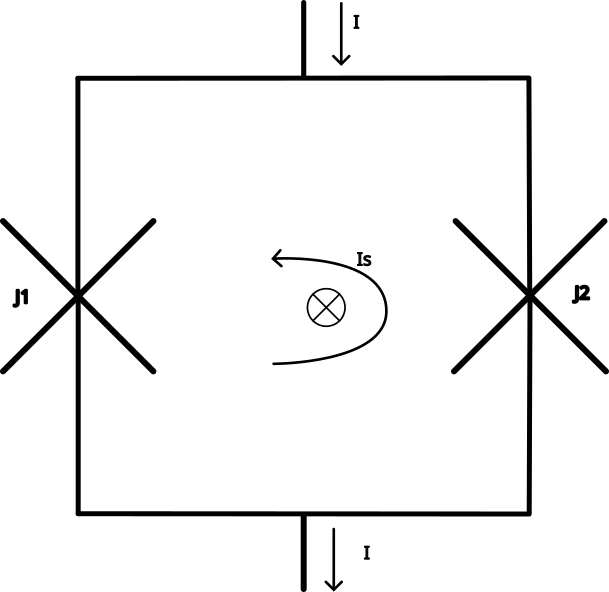
\includegraphics[width=0.3\linewidth]{SQUID}

    \caption{A circuit schematic depicting the configuration of a simple DC SQUID. The current $I$ is the bias current and the current $I_s$ is the screening current developed by an external magnetic field}
    \label{fig:squidFig}
\end{figure}

A relationship between the current and the flux through the loop of the SQUID would like to be derived. The current through each Josephson junction is denoted as $I_1$ and $I_2$ for junction 1 and 2 respectively. From figure \ref{fig:squidFig} one can easily see that there are 2 possible paths through the SQUID. Following the derivation of \cite{Feynman_Leighton_Sands_2013} one can write the change in phase through each branch of the squid using equations \ref{eq:PhaseChange1} and \ref{eq:PhaseChange2} \cite{Feynman_Leighton_Sands_2013}.

\begin{equation}
    \Delta\theta_{1} = \theta_1 + \frac{2q_e}{\hbar}\int_{\text{left branch}} \Vec{A}\cdot d\Vec{s}
    \label{eq:PhaseChange1}
\end{equation}

\begin{equation}
    \Delta\theta_{2} = \theta_2 + \frac{2q_e}{\hbar}\int_{\text{right branch}} \Vec{A}\cdot d\Vec{s}
    \label{eq:PhaseChange2}
\end{equation}
Where $\theta_1$ and $\theta_2$ is the change in phase across their respective junctions. Similarly, $\Delta\theta_1$ and $\Delta\theta_2$ refer to the change in phase through the left and right branch respectively. As previously discussed, the integral of the phase gradient around a closed loop must be an integer multiple of $2\pi$. As a consequence, subtracting equation \ref{eq:PhaseChange2} from \ref{eq:PhaseChange1} must yield $2\pi n$. Using equation \ref{eq:intCurrent} we derive equation \ref{eq:loopInt}.

\begin{equation}
    \theta_2  = \theta_1 - 2\pi n + \frac{2q_e}{\hbar}\Phi
    \label{eq:loopInt}
\end{equation}

Using equation \ref{eq:joseph}, \ref{eq:loopInt} and a KCL at the top or bottom node, the relation between the current going into the loop and the flux through the loop is derived and equation is found. Here the $2\pi n$ term can be neglected as a $2\pi n$ shift in phase does not change the value of the function. 

\begin{equation}
    I = I_2sin(\theta_2) + I_1sin(\theta_2 - \frac{2q_e}{\hbar}\Phi)
    \label{eq:squidI}
\end{equation}

Equation \ref{eq:squidI} describes the general behaviour of the DC SQUID. The current voltage characteristics are shown in the figure below \textcolor{red}{Get figure} \newline
It is worth pointing out the mechanism through which flux is quantized in the SQUID loop. When an external field is applied to the washer a screening current begins to flow around the loop to oppose the applied field. The magnitude of the current is determined by the loop inductance. Assuming that the applied flux density is constant throughout the hole in the loop, the magnetic flux generated by the screening current is $\Phi_s = LI_s$. The total flux in the loop is $\Phi_{\text{ext}} + \Phi_{s} = n\Phi_0$. If applied flux is less than $\frac{\Phi}{2}$ the screening current flows to oppose the build up of flux in the loop by ensuring that $\Phi_s = -\Phi_{\text{ext}}$ and thus the total flux in the loop is 0. When the applied flux increases to $\frac{\Phi}{2}$ the flux state of the loop changes and the screening current changes direction \cite{Drung2016NBSQUIDS} to ensure that the total flux in the loop is $\Phi_0$. If the external flux is further increased the flux induced by the screening current decreases from $\frac{\Phi_0}{2}$ to $0$ such that the total flux in the loop remains $\Phi_0$. The trend continues as the external field strength is increased. Because of this mechanism the critical current and voltage-flux characteristics of the SQUID always has a period of $\Phi_0$ \cite{SQUIDhandbook}. As pointed out by \cite{Drung2016NBSQUIDS}, this allows the SQUID to be automatically calibrated as 1 period corresponds to 1 flux quantum in the loop.

\subsection{Practical DC SQUIDS and design considerations}

\subsubsection*{The resistively shunted junction}
Practical realisation of a DC SQUID requires that the designer connect shunt resistors to each junction \cite{Drung2016NBSQUIDS}. This is done such that the system is strongly over damped \cite{SQUIDhandbook}. In the context of the discussion on the I-V characteristics  of the Josephson junction the addition of the shunt resistors correspond to the effect of the junction capacitance becoming negligible. In the absence of a shunt resistor the I-V characteristics of a Josephson junction has hysteresis \cite{Drung2016NBSQUIDS}. 

\subsubsection*{Effective Area and Inductance}
Two important quantities for the design and analysis of SQUID sensors are the effective area and the SQUID inductance. The effective area of a SQUID washer is defined as \cite{SQUIDhandbook}:

\begin{equation}
    A_{\text{eff}} = \frac{\Phi_s}{B_a}
    \label{eq:effArea}
\end{equation}
In equation \ref{eq:effArea} $\Phi_s$ refers to the flux coupled into the SQUID loop as a result of an applied magnetic field $B_a$. The effective area is typically higher than the geometric area of the washer hole due to the Meissner effect \cite{Drung2016NBSQUIDS}. As will be shown in the next section there is a limit on the inductance of a SQUID loop and by extension a limit on how large one can make a SQUID. Critically, the field sensitivity is inversely proportional to the effective area. The magnetic field noise is inversely proportional to the geometric area of the hole in the SQUID loop. The design then comes down to creating a SQUID loop that maximises the effective area but minimizes the actual area of the SQUID loop to keep the SQUID loop inductance and thus the field noise to a minimum \cite{SQUIDhandbook}.

\subsubsection*{The uncoupled SQUID}
Below is an example of an uncoupled DC SQUID structure. 
\begin{figure}[h]
    \centering
    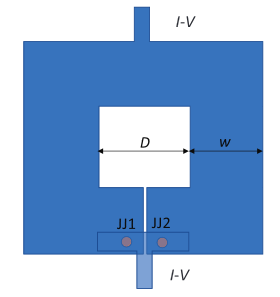
\includegraphics[width=0.4\linewidth]{UncoupledSQUID}
    \caption{A diagram of a practical uncoupled DC SQUID structure \cite{DCSQUIDdesignImage}}
    \label{fig:UncoupledSQUID}
\end{figure}
The uncoupled SQUID is the simplest of designs as it only consists of a single superconducting loop with 2 resistively shunted Junctions. The SQUID characteristics are determined by the loop inductance, critical current, shunt resistance and parasitic junction capacitance \cite{Drung2016NBSQUIDS}. Design involves choosing the optimal set of these parameters to satisfy the design requirements. This is often not a trivial task due to the non-linear nature of the equations describing the behaviour of the Josephson junction and by extension the DC SQUID. Through extensive simulation a number of key design parameters have been identified \cite{Drung2016NBSQUIDS}. The first of which is described by equation \ref{eq:NoisePar} and is referred to as the noise parameter \cite{SQUIDhandbook}. 
\begin{equation}
    \Gamma = \frac{2\pi k_bT}{\Phi_0I_c}
    \label{eq:NoisePar}
\end{equation} 
The noise parameter is the quotient of the thermal energy and the Josephson coupling energy \cite{SQUIDhandbook}. It has the effect of an apparent reduction in the critical current of a junction at low voltages \cite{Drung2016NBSQUIDS}. \newline
The second design consideration is the quality or "Q" factor. For currents the phase shift induced by the Josephson junction can be interpreted as an inductor \cite{SQUIDhandbook}. Under this approximation it is clear to see how the combination of the shunt capacitance and junction create an RC resonator. As pointed out by \cite{Drung2016NBSQUIDS} it is often desirable to keep the quality factor of resonating circuits in non-linear systems close to unity. This leads to the next design rule \cite{SQUIDhandbook}:
\begin{equation}
    \beta_c = Q_j^2 = 2\pi I_cR^2\frac{C}{\Phi_0} \approx 1
    \label{eq:QFACT}
\end{equation}
This parameter is largely controlled by designer by tuning the shunt resistance.\newline
The next design rule sets a constraint on the choice of L (the inductance of the SQUID washer). The magnitude of the screening current in the loop is related to the applied flux through the inductance of the SQUID washer. Increasing the SQUID loop inductance results in a smaller screening current induced in the loop to keep the flux in the loop at an integer multiple of the flux quantum. This leads to a smaller modulation depth of the critical current and by extension the modulation depth of the voltage flux characteristic of the SQUID \cite{Drung2016NBSQUIDS}. For this reason it is generally better to keep the inductance of the SQUID washer low. Simulations have shown that for very low inductances the SQUID noise increases, so a compromise is in order \cite{Drung2016NBSQUIDS} leading to the next design rule: 
\begin{equation}
    \beta_L = \frac{2LI_c}{\Phi_0} \approx 1
    \label{eq:SQUIDmodDepth}
\end{equation}

\subsubsection*{Coupled SQUIDS}
\textcolor{red}{See pg 177}

\subsubsection*{SQUID readout}
\textcolor{red}{See pg 139 of SQUID hb}
\section{Noise in SQUIDS}
The importance of understanding, modelling and predicting the noise energy of a SQUID design cannot be understated. A reduction in flux noise necessarily increases the sensitivity of a SQUID system. As reported by \cite{LowNoiseGrad} a typical commercially available SQUID system can achieve magnetic field resolutions of $5 \si{fT/Hz}$. Experimental results suggest that the current consensus on the origin of white noise is in agreement with the theory, that is the origin of the noise is known. The theory explains the white noise as thermal noise and the statistical properties are usually well known \cite{Drung2016NBSQUIDS} \cite{SQUIDhandbook}. For frequencies greater than about $10 - 100\si{Hz}$ the thermal noise dominates. Below $10 - 100\si{Hz}$ the so called $1/f$ noise dominates \cite{DCSQUIDdesignImage}. Unlike thermal noise no consensus has been found on the origin of $1/f$ noise. According to \cite{SQUIDhandbook}, in the fields of biomagnetism and geophysics the low noise properties of SQUIDS must extend to frequencies below $1\si{Hz}$. Furthermore, \cite{QubitPerf} reports the primary cause of decoherence in frequency tuneable quits is the so called $1/f$ flux noise, once again highlighting the important role $1/f$ flux noise has.


\subsection{1/f flux noise}
Although there is no consensus on the exact origin of $1/f$ noise many agree that the origin of the excess noise at low frequencies is due to randomly reversing of magnetic moments distributed thinly on the surface of a super conductor \cite{FluxNoiseCol}. As \cite{FluxNoiseCol} reports the noise has a power spectral density of the form of equation \ref{eq:PSDnoise}.
\begin{equation}
    S_\Phi(f) = \frac{A}{f^\alpha}
    \label{eq:PSDnoise}
\end{equation}
The parameter A is insensitive to the geometry and materials of the substrate \cite{fluxNoiseSquidsStevenAnton}. The parameter $\alpha$ is the slope of the noise on a log-log plot. In \cite{SurfaceSpinOrig} the authors propose that the origin of magnetic moments on the surface of the superconductor can be attributed to $O_2$ molecules absorbed on the surface. In \cite{OriginAndReductionOf1/fNoise} the authors provide further supporting evidence to the claims of \cite{SurfaceSpinOrig} by investigating the effect of surface treatments on low frequency flux noise. They found that surface treatments as well as a better sample vacuum environment led to significant improvement in low frequency flux noise. Experimental results suggest the spin density on the surface of the superconductor to be $5\times10^{17}m^{-2}$. According to \cite{fluxNoiseSquidsStevenAnton} various authors have characterized the noise due to surface spins by calculating the mean square flux noise ($\langle \Phi^2\rangle $). The authors make use of a model where spins are independently and identically distributed with each spin having a magnetic moment equal to the Bohr magneton ($\mu_B$). The results correlated with experimental evidence as it conformed to the properties of the power spectral density one expects from the low frequency flux noise \cite{fluxNoiseSquidsStevenAnton}. Specifically, the models conformed to the property that the magnitude of the flux noise is a weak function of the geometry of the SQUID.

\subsection{Techniques for predicting mean square flux noise}
\label{subsec:PredictFluxNoise}
The importance of being able to predict the low frequency flux noise in SQUID's has led many to attempt to predict it using the mostly agreed upon model of magnetic defects on the surface of the super conductor.

\textcolor{red}{Change title}
\subsubsection*{Numerical method by Bialczak et al.}
In the work done by Bialczak et al. \cite{BialczakTestLoop}, the authors describe how they calculate the mean square flux noise due to a random distribution of surface defects on the substrate of the SQUID. Critically, the authors do not make the assumption that defects are confined to the surface of the superconducting film. In this method a test loop is used to represent a surface defect. The test loop is dimensioned such that the product of the area of the loop and the current in the test loop is equal to the Bohr magneton. The authors used FastHenry to calculate the mutual inductance between the SQUID and the test loop. Once the mutual inductance is known, one can simply relate it to the flux coupled into the loop by a single magnetic moment by multiplying the test current by the mutual inductance \cite{BialczakTestLoop}. 
\begin{equation}
    \Phi_s = M(x,y)I
    \label{eq:FluxCoupleBial}
\end{equation}
The method requires a new simulation to be run for each location and orientation of the test loop. This is computationally taxing and severely limits the resolution and accuracy of the calculation \cite{fluxNoiseSquidsStevenAnton}. Despite the heavy computational cost of the method it is fairly general and can easily be extended to different geometries. In theory this method could be used to verify the validity of the theoretical model because, given a powerful enough computer, one could perform an exact simulation, neglecting the error due to meshing, where the test loop is dimensioned such that it is on the order of a single surface defect. The authors found that the results they obtained from their numerical model match best when an areal spin density of $5\times10^{17}\si{m^{-2}}$

\subsubsection*{The analytic method of Koch et al.}
The approach taken by \cite{KochModel} attempts to derive analytic solutions for the mean square low frequency flux noise in a SQUID. In \cite{KochModel} the authors examine a theoretical model where the flux noise is a result of two-level state (TLS) defects in the oxides of the superconducting film \cite{KochModel}. A TLS defect is a microscopic defect that can be described by a two-state quantum system \cite{KochModel}. The defects can in principle be any plausible two state quantum system but in \cite{TLSDefectExplanation} the authors list the following as examples of such defects:
\begin{center}
    \begin{itemize}
        \item Tunnelling atoms \\
        \item Dangling electronic bonds \\
        \item Surface impurities \\
        \item Trapped charges \\
    \end{itemize}
\end{center}
To derive an analytic solution for the mean square flux noise figure one has to make assumptions about the nature of the TLS defects. In \cite{KochModel} the assumption that all defects have a magnetic moment equal to the Bohr magneton, the assumption that defects are uniformally distributed across the surface of the superconducting film and the assumption that the magnetic moments of the defects are randomly orientated is made. \par
We start by recognizing that the mutual inductance between any 2 arbitrarily shaped loops in space is equal. That is the inductance matrix is of the form: 
\begin{equation}
    \begin{bmatrix}
        \lambda_1 \\
        \lambda_2 \\
    \end{bmatrix} 
    = 
    \begin{bmatrix}
        L_1 && M \\
        M && L_2 \\
    \end{bmatrix}
    \begin{bmatrix}
       I_1 \\
       I_2 \\
    \end{bmatrix}
    \label{eq:InductanceMatrix}
\end{equation}
The inductance is a function of the geometry of the problem and is therefore independent of the flux and current terms \cite{Feynman_Leighton_Sands_2013}. If one sets $I_2 = 0$ and $I_1 = I'$ it is easy to solve for the mutual inductance: 
\begin{equation}
    M = \frac{\lambda_2}{I'}
    \label{eq:Mutual2}
\end{equation} 
Doing the same but this time setting $I_1 = 0$ and $I_2 = I'$:
\begin{equation}
    M = \frac{\lambda_1}{I'}
    \label{eq:Mutual1}
\end{equation}
Because $M$ is constant in both equations \ref{eq:Mutual1} and \ref{eq:Mutual2}, $\lambda_1$ must equal $\lambda_2$. This demonstrates the principle of reciprocity. Clearly it does not matter which loop is excited by the current $I'$ the flux remains the same in both cases. This is leveraged by \cite{KochModel} because unlike the method employed by Bialczak et al. \cite{BialczakTestLoop}, the test loop becomes the SQUID washer as the flux coupled into the washer due to a magnetic moment is the same as the flux coupled into the area of a magnetic moment (defined as $\Vec{\mu} = \Vec{S}\cdot I$ where S refers to the vector area) due to a test current in the SQUID washer. \par
For a thin wire of diameter $D$ and loop radius $R$, the magnetic field on the surface and tangent to the circular cross-section of the wire is approximated for a large loop radius by applying the ampere circuital law. We choose a path of integration around the diameter of the wire such that the assumption that the magnetic flux density tangent to the cross-section of the loop is constant can be made. Under these assumptions' equation \ref{eq:BField} is found.
\begin{equation}
    B = \frac{\mu_0I}{\pi D}
    \label{eq:BField}
\end{equation}
Following the law of reciprocity we can express the flux through the loop due to a surface defect randomly orientated on the ring at a position $\Vec{r}$:
\begin{equation}
    \Phi = \Vec{\mu_B}\cdot \frac{B(\Vec{r})}{I} 
    \label{eq:Flux}
\end{equation}
The defects are uniformally distributed, so the number of magnetic moments is simply $\sigma 2\pi^2RD$.

\begin{equation}
    \langle \Phi^2 \rangle = \frac{\mu_B^2 \mu_0^2}{\pi^2 D^2}\cdot\langle (\Vec{a_m}\cdot \Vec{a_\text{bfield}(\Vec{r})})^2\rangle \cdot \text{Surface area of the loop} \cdot \sigma
    \label{eq:MSFN}
\end{equation}
Here $\Vec{a_m}$ is a random unit vector representing the direction the magnetic moment is pointing and $\Vec{a_b(\Vec{r})}$ represents the direction of the b field as a unit vector. Trivially, the expectation of the dot product between a unit vector and a random unit vector in $\mathbb{R}^3$ (assuming the random vector has a uniform distribution) evaluates to $\frac{1}{3}$. Simplifying equation \ref{eq:MSFN} and applying this result equation \ref{eq:MSFNfinal}.

\begin{equation}
    \langle \Phi^2 \rangle = \frac{2\mu_0^2\mu_B^2\sigma R}{3D} 
    \label{eq:MSFNfinal}
\end{equation}
This is the same result as found in \cite{KochModel}. Using the same technique \cite{KochModel} derives the equation for the mean square flux noise in a thin film circular loop of radius $R$ and track width $W$ to be:
\begin{equation}
    \langle \Phi^2 \rangle \approx \frac{2\mu_0^2\mu_B^2}{3}\sigma\frac{R}{W}[\frac{\text{ln}(\frac{2bW}{\lambda^2}) }{2\pi}+ 0.27] 
    \label{eq:ThinFilmMSFN}
\end{equation}
The authors concluded that the standard TLS model incorrectly describes the mechanism through which low frequency 1/f flux noise arises. Despite this conclusion, the analytical methods used by \cite{KochModel} is valuable as the use of the principle of reciprocity is the key to the next method used to calculate mean squared flux noise figures.

\subsubsection*{The numerical method of S.M. Anton et al.}
This method follows on closely from the method employed by \cite{KochModel}. In \cite{fluxNoiseSquidsStevenAnton} the same assumptions are made about the nature of the surface defects as in \cite{KochModel}. This technique takes the analytical method demonstrated by \cite{KochModel} and implements it numerically. To do this \cite{fluxNoiseSquidsStevenAnton} makes use of a superconducting version of FastHenry to compute the current distribution due to a time varying voltage source applied to a test port on the SQUID washer as shown in figure \ref{fig:WASHERSteven}.
\begin{figure}[h]
    \centering
    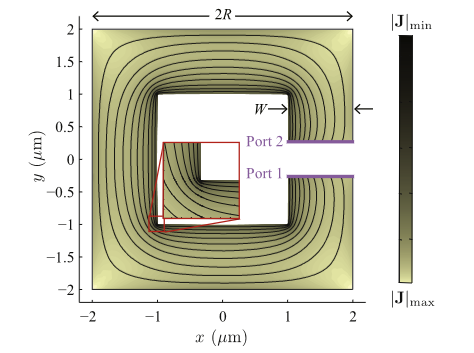
\includegraphics[width=0.5\linewidth]{Washer}
    \caption{A figure produced by \cite{fluxNoiseSquidsStevenAnton} showing the use of a test port on the SQUID washer}
    \label{fig:WASHERSteven}
\end{figure}
The author noted that the time complexity of FastHenry at the time was roughly $\mathcal{O}(N_{\text{seg}})$, where $N_{\text{seg}}$ refers to the number of segments in the mesh. FastHenry did not support a meshing scheme where segments could have varying segment widths \cite{fluxNoiseSquidsStevenAnton}. The author concluded that in order to make the computational load reasonable while still capturing the rapidly varying nature of the current distribution localized to specific regions of the geometry, a new meshing scheme needs to be developed \cite{fluxNoiseSquidsStevenAnton}. To solve this problem the author made use of the software package InductEx to create an optimized mesh where the mesh size is tuned to ensure that the change in current density from one mesh element to the next never exceeds a certain threshold. Once the current distribution is known, the magnetic field on the surface of the SQUID can be calculated using the law of Biot and Savart \cite{fluxNoiseSquidsStevenAnton}:
\begin{equation}
    \Vec{B(\Vec{r})} = \frac{\mu_0}{4\pi}\sum_{\text{sll segments}}[J_n\times\int_{V_n}\frac{\Vec{s}\cdot d\Vec{V}}{|\Vec{s}|^3}]
    \label{eq:BiotSavart}
\end{equation}
The current is assumed to be constant throughout each individual segment so $J_n$ is taken out of the integral in equation \ref{eq:BiotSavart}. This allows the integral to be solved analytically as it only depends on the geometry of a segment and not the current distribution \cite{fluxNoiseSquidsStevenAnton}. Once the magnetic flux density on the surface of the conductor is found, the principle of reciprocity can be used to calculate the mean square flux noise. In \cite{fluxNoiseSquidsStevenAnton} equation \ref{eq:MSFNfromBfield} is listed.
\begin{equation}
    \langle \Phi^2 \rangle = \frac{N\mu_B^2}{3I^2}\langle \Vec{B}^2(\Vec{r}) \rangle
    \label{eq:MSFNfromBfield}
\end{equation}
In conclusion, the author reduces the problem of calculating the mean square flux noise to finding the average magnetic flux density on the surface of the conductor. A detail that is worth mentioning is that the number of spin densities $N$ in equation \ref{eq:MSFNfromBfield} is considered large enough such that one can make a continuum approximation \cite{fluxNoiseSquidsStevenAnton}.


\graphicspath{{solutiondevelopment/fig/}}

\chapter{Solution development}
\label{chap:solutiondevelopment}
The goal of this project is to develop a tool for calculating the low frequency mean square flux noise figure given a SQUIDs geometry with the use of the software package InductEx. In \cite{fluxNoiseSquidsStevenAnton} the authors propose a framework for implementing such a tool but then only applied the method to a square washer. As pointed out in \cite{fluxNoiseSquidsStevenAnton} the other numerical technique suffers from performance and resolution problems. This section will serve to communicate the design effort by systematically breaking down the problem and motivating design decisions along the way. I will start by first identifying the design requirements.

\section{Design goals}
\label{chap:dgoals}
In section \ref{chap:litreview} it was made clear that the origin of the low frequency noise is still unknown. The S.M. Anton et al. pointed concluded \cite{fluxNoiseSquidsStevenAnton} by remarking on the flexibility of his numerical framework. It can readily be adapted, with only minor modifications to the framework, to account for a variety of different models. As such a major design requirement is to reflect the flexibility of the framework within the design of the tool.
The second and perhaps most obvious design goal is that the tool must be fast. The end user of such a tool is a SQUID designer. As discussed in chapter \ref{chap:litreview} the design of SQUID systems relies heavily on computational methods. The non-linear nature of the Josephson junctions makes analytical solutions to design problems not feasible. In such cases the designer often has to rely on an iterative approach to design.
The tool must be generalized to work on any geometry one might give it.
The last design goal is to use TetraHenry for the calculation of the magnetic flux density. 

\section{High Level System Design}
\label{chap:high level design}
The project calls for the development of 2 independent modules. The first module must implement mesh refinement around regions of rapidly varying currents across mesh nodes. The second module must implement the numerical framework as described by \cite{fluxNoiseSquidsStevenAnton} using the simulation results from InductEx and TetraHenry. \par
To understand the role the tool will play one must first understand the basic interactions a user might have with the software package. One must also understand what each entity requires as input and what its outputs are. Figure \ref{fig:Inductexproc} summaries this and figure \ref{fig:ProcessFlow} shows how each module interacts with this process.
\begin{figure}[h]
    \centering
    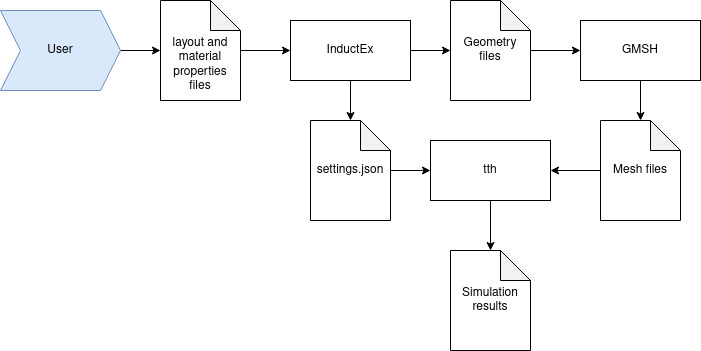
\includegraphics[width=0.8\linewidth]{Inductexproc}
    \caption{A process showing how the average user might interact with InductEx and TetraHenry. The figure also shows typical input and output files at each entity in the process.}
    \label{fig:Inductexproc}
\end{figure}
\begin{figure}[h]
    \centering
    \includegraphics[width=0.8\linewidth]{ProcessFlow}
    \caption{A process chart showing how the user interacts with InductEx as well as how each module will interact with this process.}
    \label{fig:ProcessFlow}
\end{figure}

\subsection{InductEx}
InductEx has gone through major changes since the publication of \cite{fluxNoiseSquidsStevenAnton}. InductEx is a powerful tool that supports a large feature set. Most of these features are not relevant to this project. I only require magnetic field calculations and current distribution for the surface of the conductor, so these features will mostly be ignored.

\subsection{GMSH}
GMSH is an open-source tool that is used to discretize geometry \cite{GMSH}. GMSH supports a scripting language to specify geometry before discretization. InductEx generates a file in this scripting language to be run through GMSH to generate a finite element mesh for use in TetraHenry. GMSH typically accepts a ".geo" file and outputs a ".msh" file. In GMSH you specify the geometry in a hierarchical fashion. You start by defining the lowest dimension elements and build up the geometry from there. In GMSH the lowest dimension entity is the point and is referred to as a "0 dimensional" entity. Higher dimensional entities are bounded by lower dimensional entities for example: A volume is bounded by a set of 2 dimensional surfaces. A surface is defined by a closed loop of 1 dimensional curves. A curve is defined by the 0 dimensional points. This fact will become useful in the design of the GMSH extraction module. GMSH entities are added to physical groups specified by the user. Physical groups are essentially just names for collections of mesh entities. The most common use of physical groups is to use them to define material properties. The implementation and use of physical groups depend on the context GMSH is used in. In TetraHenry physical groups are used to specify a number of things but most relevant to this project, it is used to specify the mesh entities to be used for field calculations. \par

\subsection{TetraHenry (TTH)}
TetraHenry is the numerical field solver that will be used to calculate the surface magnetic flux density. This project will interact directly with TetraHenry. Refer to appendix \ref{appen:settings} for the template ".json" settings file used. Depending on the setup of the simulation, TetraHenry will write the results to a folder titled output. When specified, TetraHenry will write the magnetic flux density to a "vtk" file as an unstructured grid. TetraHenry also supports a feature where a loop can be excited by specifying a "hole" port. This eliminates the problems \cite{fluxNoiseSquidsStevenAnton} had where the current distribution was distorted around the port where the test current is injected. 

\section{Detailed Design}
\label{chap:ddesign}
\subsection{Choice of programming language}
The visualisation tool kit (VTK) is an open-source modelling and visualisation tool kit. As TetraHenry reports simulation results in the VTK file format it is necessary that the language of choice supports the VTK library. Of the rich variety of programming and scripting languages available, few match the design requirements. The VTK library is only supported by python and C++. Python is a high level interpreted language and is often used for scientific computing. Python is very flexible but suffers from performance issues due to it being interpreted. C++ is a lower level compiled programming language that is generally regarded as a "fast" programming language. This is largely due to the fact that it does not have the overhead that comes with an interpreted language. In order to meet performance goals C++ will be used.


\subsection{The mesh optimisation module}
\label{chap:meshopt}
The idea behind mesh optimisation in this context is to reduce the number of mesh elements in the resulting mesh without compromising on the accuracy of the field calculations. In the work done by Anton et al. \cite{fluxNoiseSquidsStevenAnton} an older version of InductEx was used. This version of InductEx used filaments as mesh elements. In many optimisation problems the challenge is to find a solution to said problem under some constraint. The challenge in mesh optimisation is finding this constraint. The methods employed by the authors in \cite{fluxNoiseSquidsStevenAnton} involved finding the spline interpolation of currents between adjacent nodes. The constraint was then set such that the change in current between nodes cannot exceed a user specified threshold. If adjacent mesh elements are found where this is the case the mesh elements are divided using the spline interpolation to adhere to this constraint. The new mesh is then used to solve for the current distribution and the same process is repeated until it reaches the iteration limit or the solution converges on a stable mesh (no subdivisions are made). \par
The version of InductEx this project is designed to work with supports tetrahedral meshing which is a far superior approach. As previously mentioned, all meshing is done with GMSH and as such mesh optimisation of this nature will require some form of integration with GMSH. \par
In GMSH the longest side of a mesh element (triangle) is referred to as the characteristic length. The characteristic length essentially defines how finely a geometric model is meshed. The characteristic length is therefore closely related to the number of mesh elements in the resulting mesh. Clearly this is how the mesh must be optimized. The characteristic length of each mesh element must be chosen such that a finer mesh is generated where the current varies rapidly across mesh elements. GMSH does not allow for the direct specification of mesh element characteristic lengths. The characteristic length of each element is instead specified through the following methods: 

\begin{enumerate}
    \item By specifying the characteristic lengths at each point in the geometric model. If the "\textit{Mesh.MeshSizeExtendFromBoundary}" option is set to true, the characteristic length will be interpolated between the defining points, curves and surfaces.
    \item By specifying the number of mesh elements per rotation.
    \item By specifying mesh size fields.
    \item By specifying structured meshing constraints.
\end{enumerate}
Option 3 was chosen because it provides the most control over mesh sizes and is the closest to being able to specify individual mesh element sizes. \par
A field in GMSH refers to a post-processing view. A post-processing view can be used as a mesh size field by setting it as a background mesh. The problem reduces to finding an appropriate background mesh. There are 2 quantities that can be used to generate the background mesh. The two options are using the magnetic flux density or using the current density. The choice of current density was made as it is what ultimately determines the magnetic flux density thereby eliminated compounding error caused by calculating the magnetic flux density from a crudely approximated current density distribution.
\subsubsection*{The minimum relative change approach}
This implementation took the approach of \cite{fluxNoiseSquidsStevenAnton}. Instead of using a spline interpolation I opted for a linear interpolation for performance reasons. The implementation should be flexible in case different interpolation method is found to produce far superior results. \par
In this approach the VTK library is used to parse the current distribution file generated by TetraHenry. The task is to find a suitable characteristic length for each node in a mesh element to be written to the background field. The process is explained with reference to figure \ref{fig:meshopt}.
\begin{figure}[H]
    \centering
    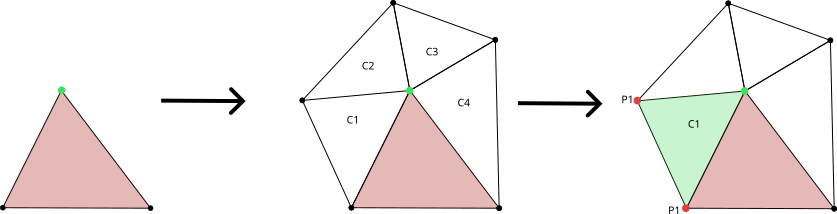
\includegraphics[width=0.9\linewidth]{meshopt}
    \caption{The figure shows the steps in the mesh optimisation algorithm when the current density is used to constrain mesh element sizes. Red region is the cell in the current iteration. The green point is the point being considered in the current iteration of looping through the points in the red region. The next step shows the mesh cells connected to the green point. The last step shows the points which will be compared to the green point. The process repeats from the second step until all cells have been explored and a maximum change of current density for the green point is found. The then algorithm reverts to the next point in the red cell and the process repeats.}
    \label{fig:meshopt}
\end{figure}
The algorithm starts by looping through every mesh element in the mesh. For a given point ($p$) in the mesh element, the VTK library can be used to find all the cells connected to point $p$. Each point in each cell is looped over to determine the maximum change in current density between point $p$ and a point connected to it. The change in magnitude between point $p$ and the point that gives the greatest change in $J$ is divided by the magnitude of the current density at point $p$ to give a percentage change in current density magnitude. The user specifies the minimum relative change allowable between adjacent nodes in the mesh. If the relative change exceeds this value it is subdivided by setting the characteristic length to a value such that, under a linear interpolation scheme and assuming that the line joining the points will be subdivided into segments equal to the characteristic length, the relative change never exceeds the minimum value between the 2 points. The values are then appended to the geometry file being optimised.

\subsubsection*{The non-linear mapping function approach}

To convert the magnitude of the current density to a characteristic length at each node a non-linear mapping is used. A linear approximation of a sigmoid function was chosen. The motivation for choosing a sigmoid function is it allows for the user to specify minimum and maximum mesh size while still interpolating between both boundaries. The approximation is used for performance reasons. Figure \ref{fig:sigmoid} shows the sigmoid and its linear approximation.
\begin{figure}[h]
    \centering
    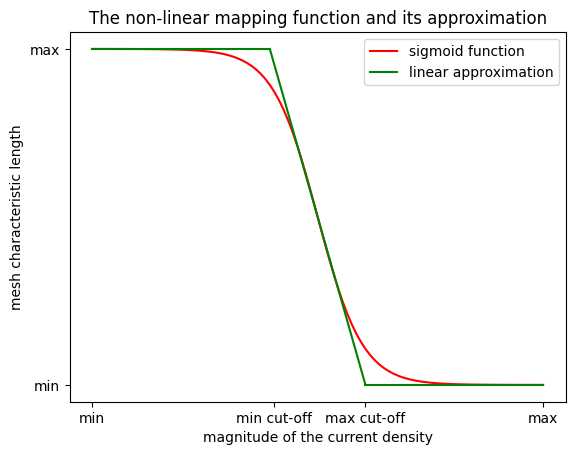
\includegraphics[width=0.5\linewidth]{sigmoid}
    \caption{A graph showing the sigmoid function with its linear approximation}
    \label{fig:sigmoid}
\end{figure}
The values that define the properties of the mapping are specified by the user. The user must specify the min cut-off, max cut-off, maximum magnetic flux density, minimum magnetic flux density, maximum characteristic length and minimum characteristic length. The module then loops through each point in the mesh and calculates the desired characteristic length from the mapping function. The background mesh is specified as a collection of triangles. Each triangle consists of three points where the characteristic length is set for each point. The background mesh is appended to the geometry file and GMSH is run to mesh the structure. 

\subsubsection*{The chosen approach}
The first option was chosen because the large number of parameters the user must specify to use the magnetic flux density is not convenient for automated testing. This is because after each mesh optimisation the values necessary to prevent over or under refinement of the mesh changes. The advantage of the non-linear mapping function approach is that it runs faster, and it provides more control over the optimized mesh. This opens the door to possible future investigations into combining the 2 approaches. 

\subsection{The noise extraction module}
\label{chap:nex}
This module is based on the work done by \cite{fluxNoiseSquidsStevenAnton}. This module will be implemented as a command line tool. The module receives the path to a VTK file which defines an unstructured grid and the total current circulating in the SQUID washer as command line arguments. The unstructured grid specifies the individual mesh elements that the surface of the SQUID washer in question consists of. Additionally, each node of each mesh element has a vector associated with it representing the magnetic flux density at the location of said node. \par
This module effectively implements equation \ref{eq:MSFNfromBfield} numerically. Expanding equation \ref{eq:MSFNfromBfield}:


\begin{equation}
    \langle \Phi ^2 \rangle = \frac{N\mu_B^2}{3I^2} \frac{\iint \Vec{B(\Vec{r})}\cdot\Vec{B(\Vec{r})} ds}{\iint ds}
    \label{eq:MSFNexpanded}
\end{equation}

Noting that in equation \ref{eq:MSFNexpanded} $N/\iint ds = \sigma$ and therefore the bottom integral can be eliminated \cite{fluxNoiseSquidsStevenAnton}. Next we discretize the integral: 
\begin{equation}
    \langle \Phi ^2 \rangle = \frac{\sigma\mu_B^2}{3I^2}\sum_{n}^{N_{\text{nodes}}}[\Vec{B}(\Vec{r_n})\cdot\Vec{B}(\Vec{r_n})]A_n
    \label{eq:MSFNdiscrete}
\end{equation}
In equation \ref{eq:MSFNdiscrete} $A_n$ refers to the area associated with the $n_{th}$ node. The method for determining $A_n$ is discussed at a later stage in the design. Similarly, $\Vec{r_n}$ refers to the vector position of the $n_{th}$ node in the unstructured grid. The basic algorithm then follows as such:
\begin{algorithm}
\begin{algorithmic}
    \State $N \gets \text{Number of points in grid}$
    \State $pts \gets \text{list of all points}$
    \State $A \gets $ list of all areas
    \State $i \gets 0$ 
    \While{$i < N$}
        \State $A_n \gets A[i]$
        \State $r_n \gets pts[i]$ 
        \State $\Phi^2 \gets \Phi^2 + \Vec{B}(\Vec{r_n})\cdot \Vec{B}(\Vec{r_n}) A_n$ 
    \EndWhile
    \State $\Phi^2 \gets \Phi^2 \cdot \frac{\sigma\mu_B^2}{3I^2}$ 
\end{algorithmic}
\caption{The algorithm for evaluating the discretized integral}
\end{algorithm}

% \subsection{Calculating the node areas}

\subsubsection*{The Choice of $\Vec{A_n}$}
Equation \ref{eq:MSFNdiscrete} shows that the calculation requires the weighted summation of the flux density over the surface. The resulting unstructured grid generated by TetraHenry associates each flux density vector with a node in the surface mesh. Figure \ref{fig:washerCloseUp} shows and example of what this looks like in practice. The challenge then is finding a scheme for choosing $A_n$.

\begin{figure}[h]
    \centering
    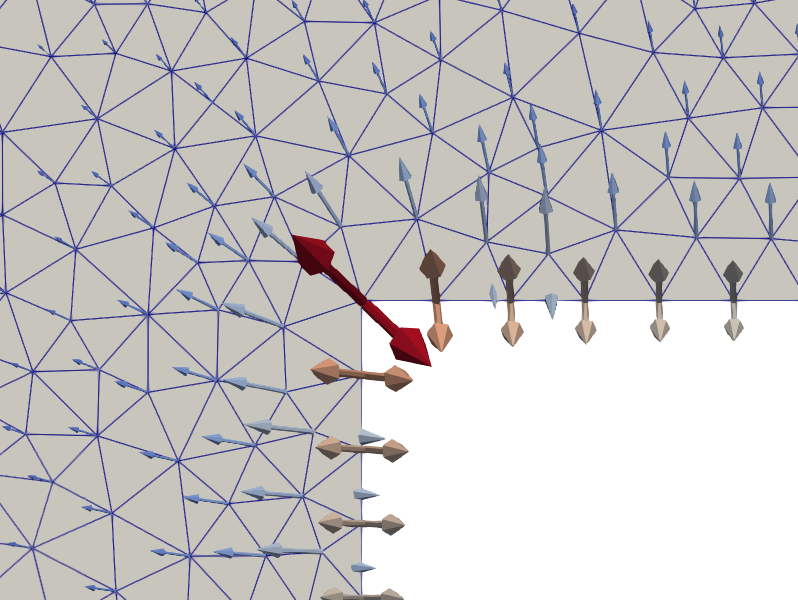
\includegraphics[width=0.5\linewidth]{washerCloseUp}
    \caption{A close up of a square washer showing the field calculations at each node in the triangular mesh.}
    \label{fig:washerCloseUp}
\end{figure}
To get some idea of what $A_n$ should look like we can investigate some of its properties. The first property of $A_n$ is expressed in equation \ref{eq:surfaceArea}.

\begin{equation}
    \text{Surface Area} = \sum_{n=0}^{N}A_n
    \label{eq:surfaceArea}
\end{equation}

The second property we would like from $A_n$ is that it minimizes the error caused by discretization. 

\begin{equation}
    ||\Vec{B_n} A_n - \iint\limits_{r \in A_n}\Vec{B}(\Vec{r})ds || = E
    \label{eq:surfaceError}
\end{equation}

It is evident from equation \ref{eq:surfaceError} that the error is $0$ when $\Vec{B}(\Vec{r}) = \Vec{B_n}$. This is not usually the case. If we assume that the mesh is fine enough such that $\Vec{B}(\Vec{r})$ varies slowly across adjacent mesh elements, we can say that the error is roughly proportional to the distance of a point in the region defined by $A_n$ to the mesh node to which $A_n$ belongs to. With this in mind we construct a new optimisation problem. \par 
Let $\Vec{X}$ be a metric space representing the surface area of the structure. We define a set of points $\Vec{P} \in \Vec{X}$ such that $\Vec{P_k}$ refers to the coordinates of the $k_{th} \in K$ node in the mesh. We would like to divide the metric space $\Vec{X}$ into $K$ regions such that each region is assigned the points closest to it thereby minimizing the error due to discretization. The $k_{th}$ region is denoted as $A_k$. Based on these arguments we can write down an objective function for this problem. The objective function quantifies the total error due to our choice of region at point $\Vec{x}$ defined by the function $t_k(\Vec{x})$.

\begin{equation}
    J = \iint \limits_{\Vec{x}\in\Vec{X}}\sum_{k}^{K}t_k(\Vec{x})||\Vec{x}- \Vec{P_k}||^2ds
    \label{eq:objFunc}
\end{equation}
The problem reduces to finding the choice of $t_k(\Vec{x})$ that minimizes $J$. The function, $t_k(\Vec{x})$ can be understood as a "label" function. It is 1 for every point $\Vec{x}$ we choose to be in region $k$ or 0 if the point is not in region $k$. The obvious choice for minimizing the sum is to set $t_k(\Vec{x})$ to zero for all $K$ regions except for the region where the distance to the point $\Vec{P_k}$ is at a minimum. Mathematically this can be expressed by equation \ref{eq:tk}

\begin{equation}
    t_k(\Vec{x}) = 
    \begin{cases}
        1 & \quad \text{If} \quad k = argmin_j\{||\Vec{x} - \Vec{P_j}||^2\}  \\
        0 & \quad \text{Everywhere else} \\
    \end{cases}
    \label{eq:tk}
\end{equation}
Recalling the definition of the Voronoi region defined in the metric space $\Vec{X}$ with the distance function $d$ and sites defined by the points $(\Vec{P_k})_{k \in K} $: 
\begin{equation}
    \Vec{A_k} = \{\Vec{x} \in \Vec{X}|d(\Vec{x},\Vec{P_k}) \leq d(\Vec{x},\Vec{P_j})\forall  j \neq k \}
    \label{eq:voronoi}
\end{equation}
If we choose the distance function in equation \ref{eq:voronoi} to be the euclidean distance we see that the regions that minimize the objective function is the Voronoi regions. \par
Choosing $A_n$ to be the Voronoi regions is a good choice not only because under the assumptions made, it minimizes the objective function but also because the triangular mesh is a Delaunay triangulation. The Delaunay triangulation is the geometric dual of the Voronoi tessellation meaning if you have the Delaunay triangulation, you have the Voronoi tessellation. This choice for $A_n$ is therefore computationally efficient. This choice also adheres to the first property we expected of $A_n$ as the Voronoi regions partition the metric space $\Vec{X}$. \par
The mesh generated by GMSH can be used to directly compute the points that define the Voronoi regions. An example is shown in figure \ref{fig:voronoi}. 

\begin{figure}[h]
    \centering
    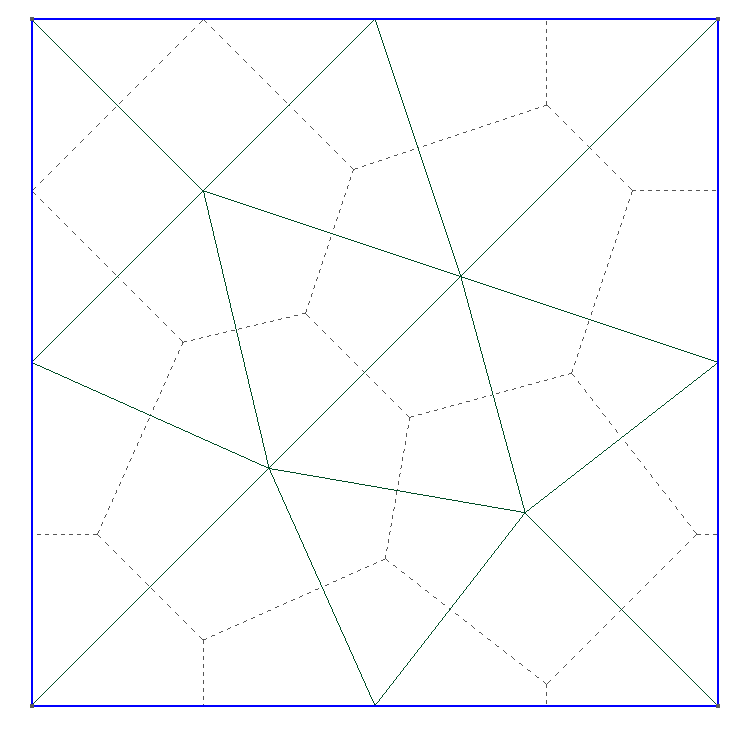
\includegraphics[width=0.3\linewidth]{voro}
    \caption{The Delaunay triangulation is shown. The triangular mesh is the solid lines. The Voronoi cells are constructed out of the dashed lines. This figure was generated with GMSH \cite{GMSH}}
    \label{fig:voronoi}
\end{figure}

These points that define the vertices of the Voronoi cells are the circumcenters of the Delauny triangulation. The algorithm follows:

\begin{algorithm}[H]
    \begin{algorithmic}
        \State $ CellList \gets $[ ]
        \For{Node $n$ in Nodes} 
            \State $C \gets $ getPointCells($n$)
            \State $V_{\text{points}} \gets $[ ] 
            \For{Cell $c$ in $C$}
                \State $P \gets $ getCellPoints($c$)
                \State $cc \gets $ computeCircumCenter($P$)
                \State $V_{\text{points}}$.pushPoint($cc$)
            \EndFor
            \State $CellList$.pushNewCell($V_{\text{points}}$)
        \EndFor
    \end{algorithmic}
    \caption{The algorithm for evaluating the discretized integral}
\end{algorithm}
When the loop exits the $CellList$ contains all the points that define the Voronoi cells. The VTK library is used to parse the simulation results. It supports optimized methods for retrieving all cells connected to a node as well as methods for fetching the points belonging to a cell. Given the position vectors $P_1$, $P_2$ and $P_3$ of the vertices of the triangle, the circumcenter ($P_c$) of a triangle arbitrarily oriented in space can be calculated using equation \ref{eq:BaryCenter}.

\begin{equation}
    P_c = \alpha P_1 + \beta P_2 + \gamma P_3
    \label{eq:BaryCenter}
\end{equation}
where 
\begin{table}[h]
    \centering
    \begin{tabular}{l}
        $\alpha = \frac{|P_2 - P_3|^2(P_1-P_2)\cdot(P_1-P_3)}{2|(P_1-P_2)\times (P_2 - P_3)|^2}$\\
        \\
        $\beta  = \frac{|P_1 - P_3|^2(P_2-P_1)\cdot(P_2-P_3)}{2|(P_1-P_2)\times (P_2 - P_3)|^2}$\\
        \\
        $\gamma = \frac{|P_1 - P_2|^2(P_3-P_1)\cdot(P_3-P_2)}{2|(P_1-P_2)\times (P_2 - P_3)|^2}$\\
    \end{tabular}
\end{table}
The perpendicular bisectors of the sides of a triangle intersect at the circumcenter, so the midpoint of each side is added to the point list of a Voronoi cell. This does not influence the shape of the cell as adjacent triangles share a side and, by the definition of a perpendicular bisector, share a perpendicular bisector. The added point is therefore collinear with the line joining adjacent circumcenters. This is done to satisfy boundary conditions. The effect of this will be discussed in more detail when the ordering of points in 3 dimensions is discussed.
\subsubsection*{The shoelace algorithm}
Now that an algorithm for choosing $A_n$ has been selected the next step is to calculate the area. If we consider an ordered set of coplanar points that define a convex N-sided polygon, the surface area of this polygon can easily be calculated using the shoelace algorithm. One property of this specific Voronoi tessellation is that the regions are always defined by convex polygons making this assumption very reasonable. Equation \ref{eq:Shoe} calculates the area given an ordered list of coplanar points $v_0, v_1, \dots, v_{N}$.

\begin{equation}
    A = \frac{1}{2}|\sum_{i=1}^{N}(v_i - v_0) \times (v_{(i+1) \% N} - v_0) |
    \label{eq:Shoe}
\end{equation}
The assumptions that all points in the Voronoi cell are coplanar and that all points are ordered does not hold. On curved surfaces or on surface edges there is more than 1 plane that the points in the cell belong to. Focusing on the assumption that all points in the Voronoi cell are co-planar, the algorithm must be able to group the points into sub cells that are coplanar. The assumption that the points are ordered will be addressed in the next section. \par
The points are read in using the VTK library triangle by triangle. Each triangular cell is read in through the "getPointCells" method. This method returns the cells that all share a point specified by an argument passed to the method. The shared point is used as the reference point. The reference point is then subtracted from every other point in the cell. The cross product of the resulting vectors is the normal to the plane that the cell is in. Due to the non-commutative nature of the cross product the order of the vectors matter. To account for this the implementation will consider both $a_n$ and $-a_n$ as the same plane. Where $a_n$ refers to a unit vector normal to the plane. The last modification that must be made is the addition of the reference point to the geometry of each sub cell. The implementation will add the reference point to each sub cell if the number of unique planes that the reference point belongs to is greater than 1. Figure \ref{fig:voroComp} demonstrates the need for this.

\begin{figure}[h]
    \centering
    \begin{subfigure}[b]{0.45\textwidth}
        \centering
        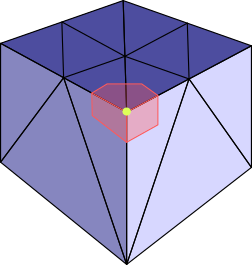
\includegraphics[width=0.5\textwidth]{vorocube}
        \caption{The Voronoi tessellation with the inclusion of the reference point}
    \end{subfigure}
    \hfill
    \begin{subfigure}[b]{0.45\textwidth}
        \centering
        \includegraphics[width=0.5\textwidth]{vorocubeWrong}
        \caption{The Voronoi tessellation without the inclusion of the reference point}
    \end{subfigure}
    \caption{The figure shows two examples of a cube. The surfaces have been meshed into triangles. The red lines indicate the boundaries of the Voronoi cell and the shaded region shows the Voronoi cell region. The yellow dot indicates the current reference point.}
    \label{fig:voroComp}
\end{figure}
The shoelace algorithm can then be performed on each individual sub cell to calculate the total area associated with a node. Figure \ref{fig:voroComp} also shows why it is necessary to add the midpoint of each side to the Voronoi cell.
\subsubsection*{Point ordering}
The points available through the "getPointCells" method in the VTK library does not have any connectivity information. That is the points are unordered. As such an algorithm needs to be developed that can generate the connectivity information after the vertex data is retrieved. The algorithm starts by defining an orthogonal basis in the plane associated with the Voronoi cell. To do this we start by taking the mean of the points and subtracting it from every point in the list. This is done so that the plane of the points runs through the origin. The next step takes the first point in the list and normalises it. This is the first vector in the orthogonal basis. The second vector is created by taking the cross product of the first vector and the normal vector of the plane. The new vector is once again normalised. By the definition of a plane the new vector has to lie in the plane. \par
Now that an orthogonal basis is established we can begin to order the points. The basic idea behind the algorithm is to take the zero mean list of points and calculate the angle between the position vectors of each point and one of the vectors in the basis set. Points are then sorted in ascending order with points with the smallest angles appearing first in the sorted list. It should be noted that this process assumes the points are co-planar, so it must be performed on a per sub cell basis. 
\begin{equation}
    \theta_i = cos^{-1}(\frac{v_i\cdot a_1}{|v_i|})
    \label{eq:angle}
\end{equation}
Equation \ref{eq:angle} calculates the angle between the $i_{\text{th}}$ point and first basis vector $a_1$. Because reflections of vectors across the axis of $a_1$ will give the same angle, there is ambiguity introduced. The sign of the dot product between each point and the second basis vector is used to resolve the ambiguity. The convention used is shown below in figure \ref{fig:planeVoro} and table \ref{tab:angles}.

\begin{figure}[h]
    \centering
    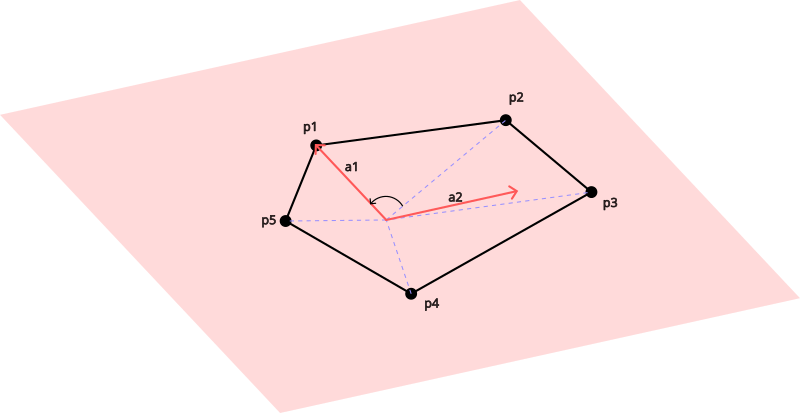
\includegraphics[width=0.5\linewidth]{plane}
    \caption{A figure showing an example Voronoi cell. Each point is labelled, and the position vectors are shown.}
    \label{fig:planeVoro}
\end{figure}

\begin{table}[h]
    \centering
    \begin{tabular}{llll}
    \hline
    Point & Angle & sign($a_2 \cdot P_i$) & Final angle \\ \hline
    p1             & 0              & +                 & 0                               \\
    p2             & 60             & +                 & 60                              \\
    p3             & 95             & +                 & 95                              \\
    p4             & 175            & -                 & 185                             \\
    p5             & 80             & -                 & 280                             \\ \hline
    \end{tabular}
    \caption{The first column refers to the point label and is a reference to figure \ref{fig:planeVoro}. The second column is the result of applying equation \ref{eq:angle}. The third column shows the sign of the projection of vector $P_i$ onto the second basis vector. The fourth column shows the angle after adjustment. The fourth column is calculated as: $360 - Angle$.}
    \label{tab:angles}
\end{table}


\graphicspath{{results/fig/}}

\chapter{Results}
\label{chap:results}
An incremental approach to testing was done for this project. Each software component was tested individually. This section will report on the results of the incremental testing as well as the results of the entire system. As a sanity check, the results will also be compared to the results in \cite{fluxNoiseSquidsStevenAnton}. Lastly the entire system will be used to calculate the flux noise power of a real SQUID design. The results will be compared to the measured noise power for each design. 
\section{The noise extraction module}
The accuracy of this module is tested by comparing its output to a numerical solution for the given geometry. This module is tested without mesh optimisation. It is tested before the mesh optimisation module because the test setup for the mesh optimisation module requires the use of the noise extraction module.
\subsection{Test setup}
The aim of this project is not to verify the numerical framework proposed in \cite{fluxNoiseSquidsStevenAnton}. The testing should reflect this. As such the test setup is designed to verify the functionality of the implementation allowing the geometry of such a setup to not be limited by realistic designs for SQUID washers. Equation \ref{eq:MSFNfinal} describes the analytical solution for a thin wire loop. The assumption made in the derivation of this equation is that $R >> D$. The test is performed was a parameter sweep from $R = \si{8}{\mu m}$ and $D = \si{5}{\mu m}$ to $R = \si{45}{\mu m}$ and $D = \si{0.4}{\mu m}$ as shown figure \ref{fig:meshedTorus}. The parameter sweep was automated using a python script.

\begin{figure}[h]
    \centering
    \begin{subfigure}[b]{0.45\textwidth}
        \centering
        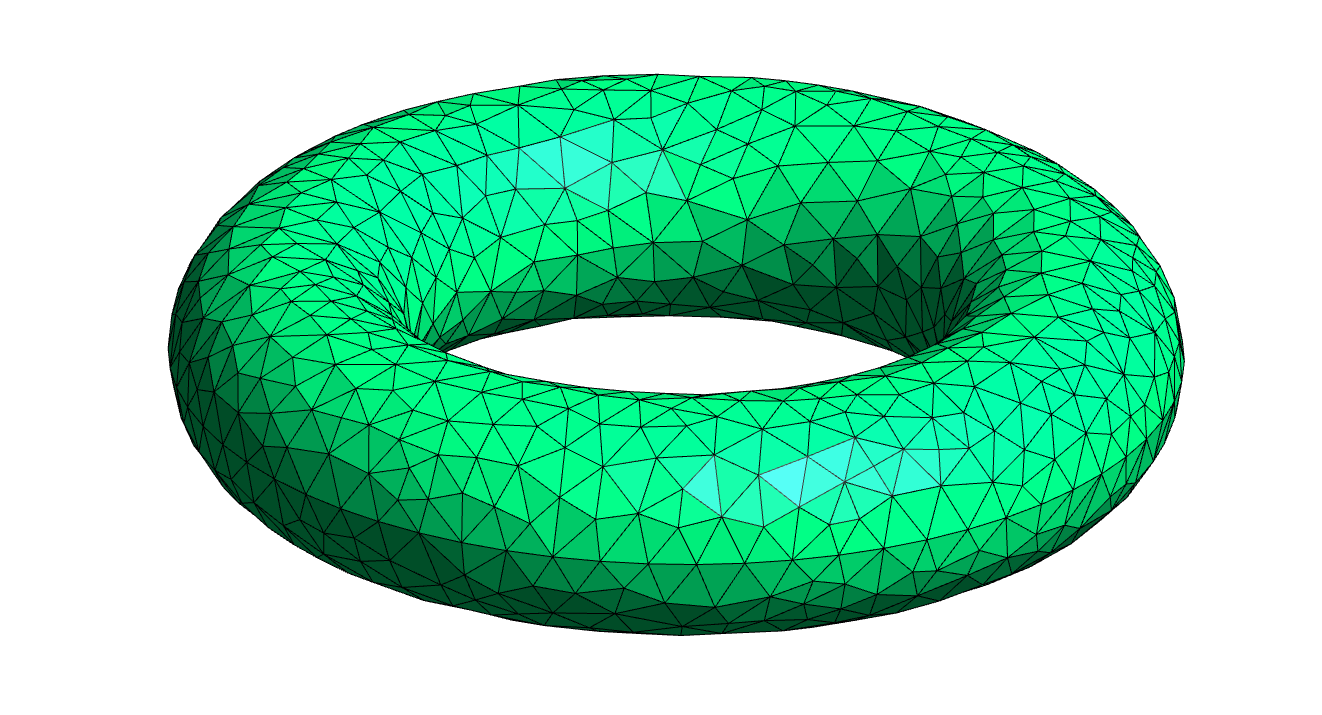
\includegraphics[width=0.5\textwidth]{torusThick}
        \caption{The meshed torus with the smallest loop radius and largest wire diameter}
    \end{subfigure}
    \hfill
    \begin{subfigure}[b]{0.45\textwidth}
        \centering
        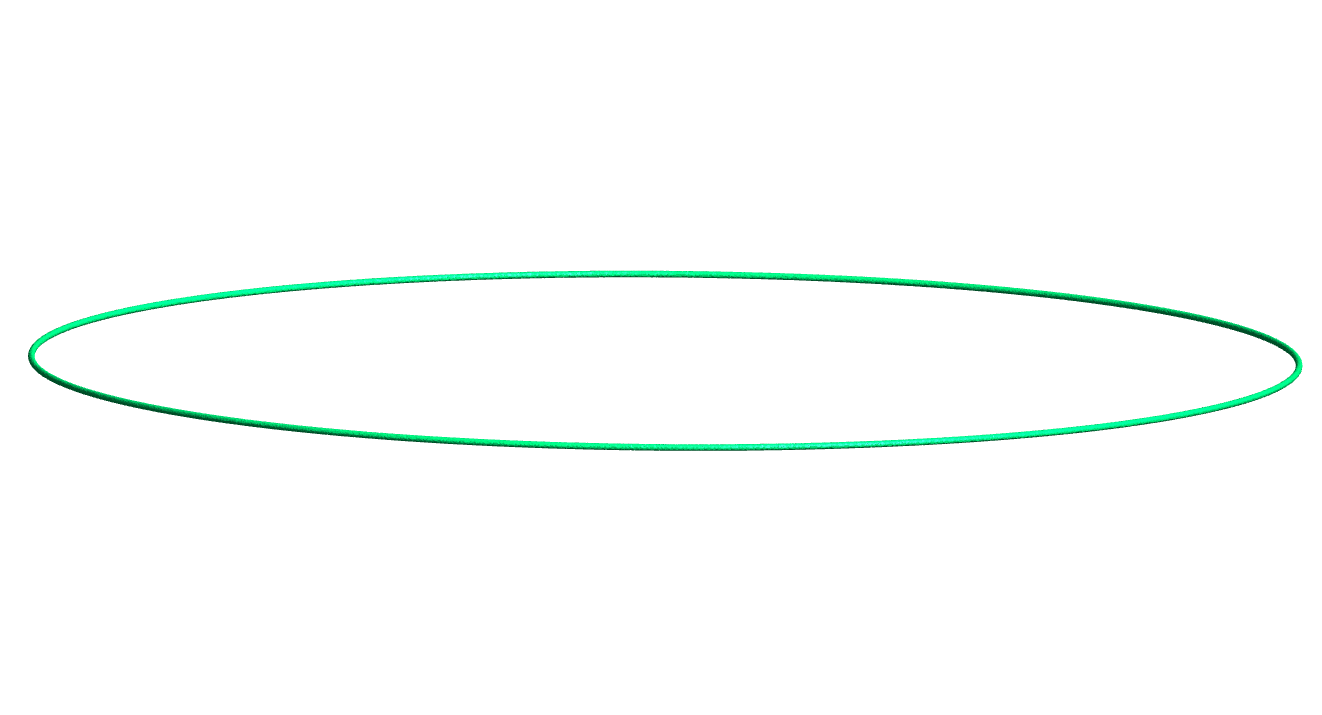
\includegraphics[width=0.5\textwidth]{torusThin}
        \caption{The meshed torus with the largest loop radius and smallest wire diameter}
    \end{subfigure}
    \caption{A figure showing the two extremes of the parameter sweep for a torus. The images show the surface mesh as generated by GMSH.}
    \label{fig:meshedTorus}
\end{figure}
\subsection{Results}

The results of the parameter sweep are summarized in figure \ref{fig:resTorus}.
\begin{figure}[H]
    \centering
    \begin{subfigure}[b]{0.48\textwidth}
        \centering
        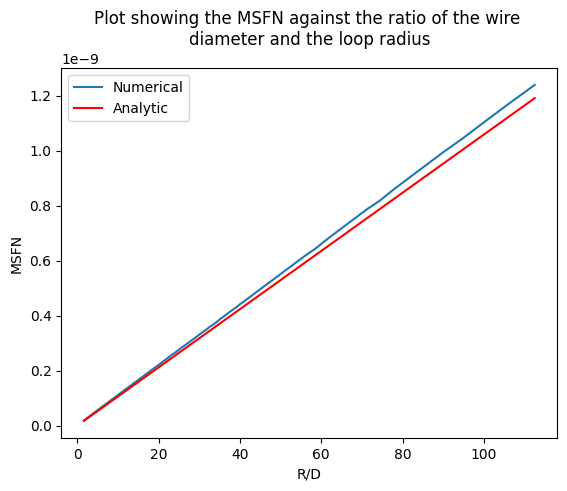
\includegraphics[width=\textwidth]{torusAVN}
        \caption{The analytical and numerical solutions for the parameter sweep}
        \label{fig:MSFNvRD}
    \end{subfigure}
    \hfill
    \begin{subfigure}[b]{0.48\textwidth}
        \centering
        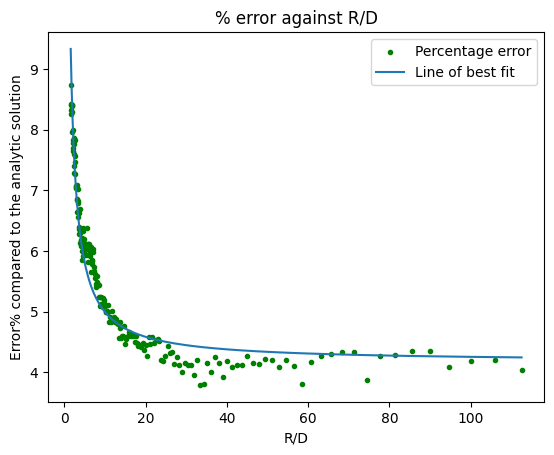
\includegraphics[width=\textwidth]{torusEVRD}
        \caption{The error plotted against the $R/D$}
        \label{fig:evRD}
    \end{subfigure}
    \caption{The figure shows both the MSFN ($\Phi_0^2 / Hz$) and the error compared to the analytic solution for the parameter sweep.}
    \label{fig:resTorus}
\end{figure}
From figure \ref{fig:resTorus} it is clear to see that the relative percentage error compared to the analytic solution decreases as the ratio of the loop radius to diameter increases. This behaviour can be attributed to the assumption: $R >> D$. The decrease in error clearly demonstrates that the noise extraction module works for this particular setup. In figure \ref{fig:MSFNvRD} the analytical and numerical results increase linearly with an increase in $\frac{R}{D}$ as expected.

\section{The mesh optimisation module}
The geometry used to test the noise extraction module is not ideal for testing the mesh optimisation algorithm. To understand why this is the case, one must consider the assumption made to derive the analytic solution. By assuming that $R >> D$ you can approximate the ring as an infinitely long wire. By extension this assumes that the magnetic flux density and current density is uniform across the surface of the ring. The testing of the noise extraction module showed that the approximation is quite good. As a consequence, the mesh optimisation algorithm does not do much because the consistent current distribution leads to the mesh being over refined everywhere or not refined at all.
\subsection{Test setup}
To test this module a thin film circular ring of loop radius $R$ and track width $W$ is used. Essentially 3 questions must be answered. How many optimisation iterations is required, how much faster the problem is solved with the optimized mesh and if the subsequent extra executions of GMSH and TetraHenry needed to optimize the mesh is worth the trouble. \par
The test setup once again consists of a parameter sweep of $R$ and $W$ over the ranges $10 \mu m \le R \le 15 \mu m $ and $  3 \mu m \le W \le7\mu m$. The two extremes of the parameter sweep is shown in figure \ref{fig:testloop}. Simulations are run at 10 linearly spaced points in these intervals. For each simulation iteration, 4 mesh optimisation iterations are run. The initial characteristic length is determined by GMSH. The average mesh element count was $1500$ elements. Testing is once again completely automated with python. At each iteration the script records a number of statistics. The script records the execution times of TetraHenry and GMSH. It keeps track of both the simulation iteration and the mesh optimisation iteration. The results are written to a CSV file to be analysed with the \textit{"pandas"} python package. 
\begin{figure}[H]
    \centering
    \begin{subfigure}[b]{0.48\textwidth}
        \centering
        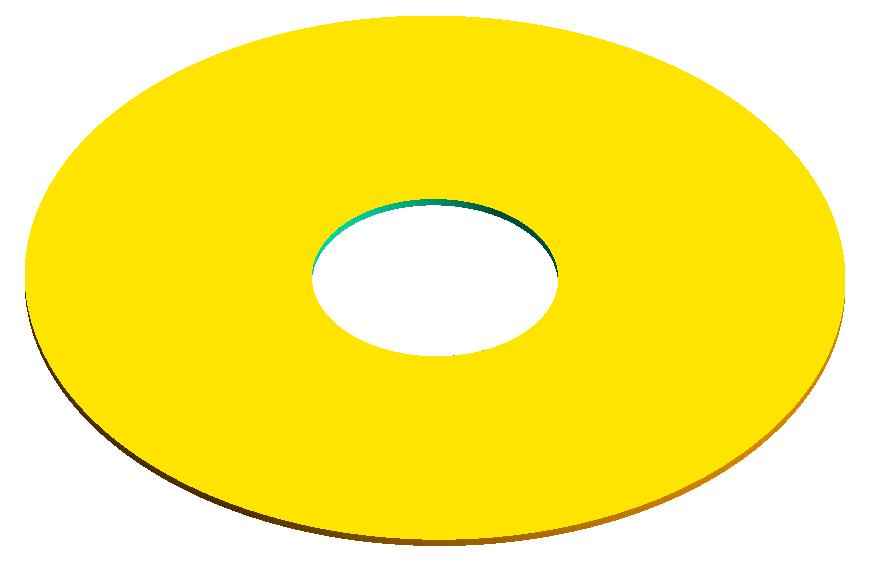
\includegraphics[width=\textwidth]{thickloop}
        \caption{The geometry of the test setup for the first iteration}
        \label{fig:thickloop}
    \end{subfigure}
    \hfill
    \begin{subfigure}[b]{0.48\textwidth}
        \centering
        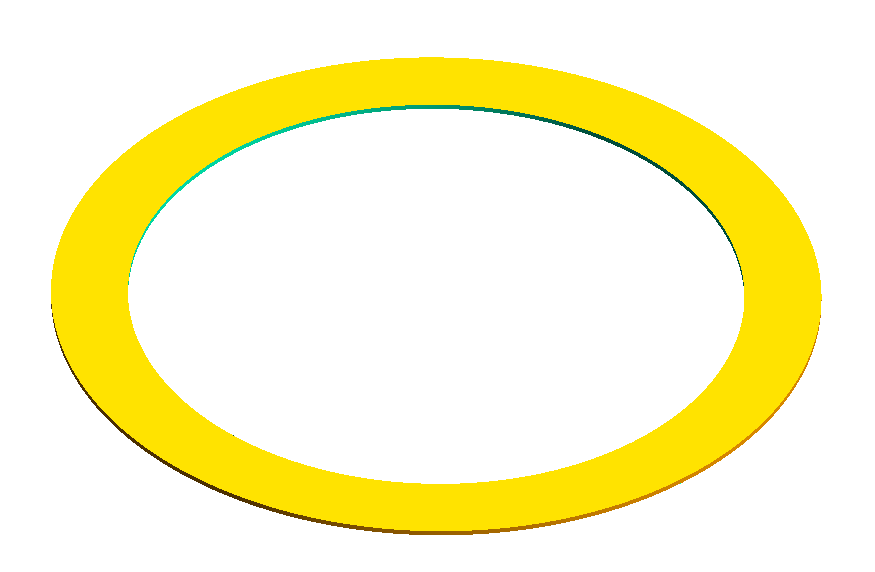
\includegraphics[width=\textwidth]{thinloop}
        \caption{The geometry of the test setup for the last iteration}
        \label{fig:thinloop}
    \end{subfigure}
    \caption{The figure shows the 2 extremes in the parameter sweep for the thin film circular loop experiment. The track thickness is set to $0.1 \mu m$}
    \label{fig:testloop}
\end{figure}
To assess the effectivity of the mesh optimisation algorithm it is necessary to make a baseline measurement. The baseline is set by forcing a minimum characteristic length in the optimized mesh and comparing the result to an unoptimized mesh with characteristic length equal to the minimum characteristic length in the optimized mesh. \par

The baseline simulations require significant computing resources and will run on a different system to the simulations with mesh optimisation enabled.
The total runtime of the baseline will be estimated. This is done by fitting a second order polynomial to the trend between the simulation time and number of nodes in the mesh. It was found through experimentation that for the specific geometry in question, the simulation time is roughly proportional to the square of the number of nodes in the mesh motivating the choice of a second order polynomial. This is necessary because simply comparing the number of nodes in both the optimized and unoptimized does not give a good indication of the difference in computational effort to solve either problems. The use of time as a metric accounts for the approximate quadratic relationship between the number nodes and the computational effort.

\subsection{Results}

To determine the number of optimisation steps necessary for convergence, the average relative error between the mean square flux noise figure calculated at each optimisation iteration and the value obtained after the $4_{th}$ optimisation iteration is calculated. The result is summarized in table \ref{tab:relerr}.


\begin{table}[H]
    \centering
    \begin{tabular}{lll}
    \hline
    Iteration number & Relative percentage error & Change in relative error \\ \hline
    0                & 1.520356                  & N/A                      \\
    1                & 0.47945                   & 1.040906                 \\
    2                & 0.028596                  & 0.450854                 \\
    3                & 0.001191                  & 0.027405                 \\
    4                & 0.000065                  & 0.001126                 \\ \hline         
    \end{tabular}
    \caption{Table of relative errors for each mesh optimisation cycle}
    \label{tab:relerr}
\end{table}

Table \ref{tab:relerr} gives some indication that after 4 iterations the solution becomes relatively stable. If we accept the 4 mesh optimisation iteration as being the correct result we can normalise the relative error and plot it against the normalised, cumulative time GMSH and TetraHenry took after each iteration. Figure \ref{fig:errvtime} shows this relationship.

\begin{figure}[H]
    \centering
    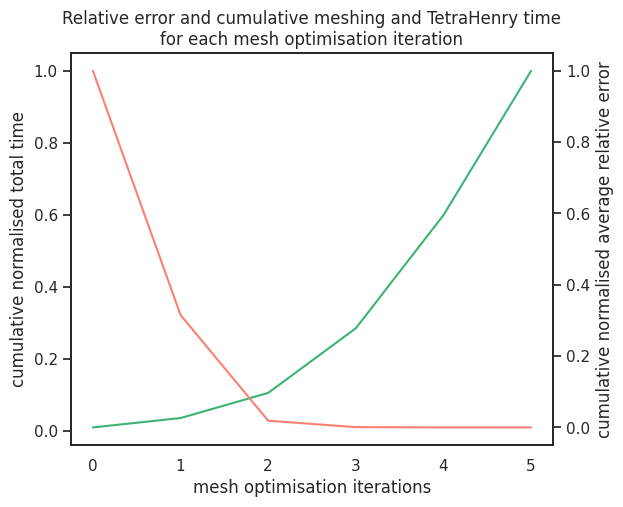
\includegraphics[width=0.5\linewidth]{errvtime}
    \caption{The figure shows the relative normalised error and the cumulative total time that GMSH and TetraHenry took at each optimisation step. The green line is the total time and the red line is the error.}
    \label{fig:errvtime}
\end{figure}

The optimal number of mesh iterations steps to minimize the time taken, and the error is between 1 and 2 iterations. The choice ultimately comes down to how accurate the user would like the solution to be. To compare the optimized mesh performance to the baseline, 2 will be selected as the optimal number of iterations.

\begin{figure}[H]
    \centering
    \begin{subfigure}[b]{0.48\textwidth}
        \centering
        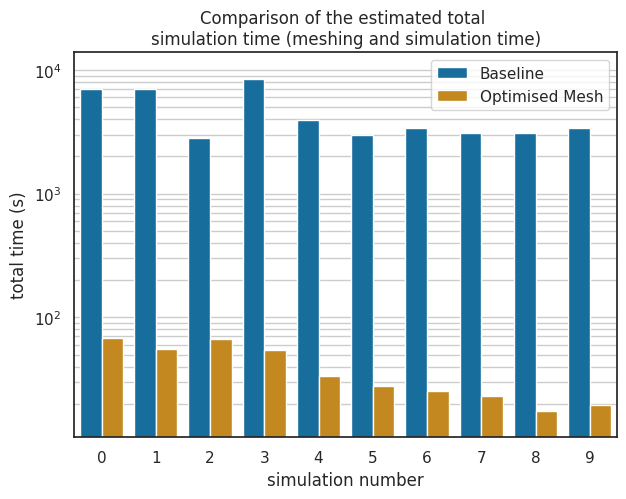
\includegraphics[width=\textwidth]{timevsimnum}
        \caption{The estimated time plotted for each simulation}
        \label{fig:timevssinnum}
    \end{subfigure}
    \hfill
    \begin{subfigure}[b]{0.48\textwidth}
        \centering
        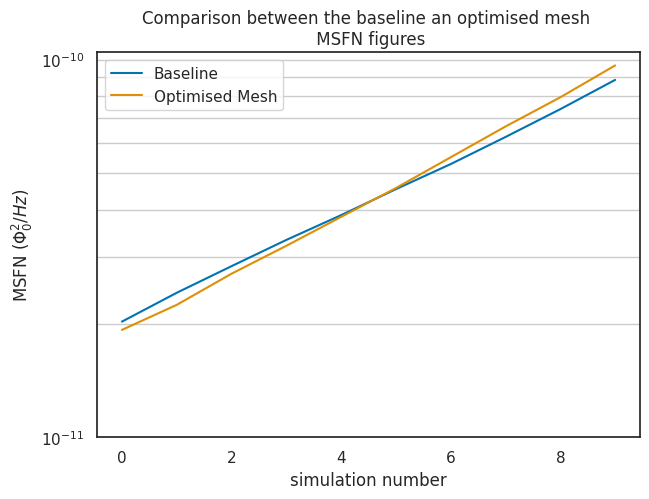
\includegraphics[width=\textwidth]{msfnvssimnum}
        \caption{The MSFN figure plotted for each simulation}
        \label{fig:msfnvssimnum}
    \end{subfigure}
    \caption{The figure shows the comparisons used to determine the accuracy and performance of the optimized mesh.}
    \label{fig:resCompOpt}
\end{figure}

Figure \ref{fig:timevssinnum} shows the estimated time to complete each simulation for the baseline as well as the optimized mesh. The result is plotted on a logarithmic scale. To estimate the time taken for the entire mesh optimisation process, the sum of the number of nodes in the mesh at each optimisation iteration is used. Figure \ref{fig:timevssinnum} shows the performance benefits of using the mesh optimisation module. On average, the computation time is decreased by a factor of 120. The best performance of the optimisation module decreased the computation time by a factor of 180 and the worst by a factor of 42. From this analysis it is clear that the mesh optimisation module provides major performance benefits. \par
Figure \ref{fig:msfnvssimnum} is used to determine the effect that optimisation has on the accuracy of the resulting MSFN figure. The relative error for each simulation is used to assess the accuracy. The average relative error was $4.86\%$. The minimum and maximum relative error was $0.66\%$ and $8.42\%$ respectively. Figure \ref{fig:msfnvssimnum} shows the optimized mesh follows the same trend as the baseline. A maximum error of $8.42\%$ is acceptable when the performance benefits of using the mesh optimisation module is considered.

\section{Comparison with the results of S.M. Anton \textit{et al.}}
\subsection{Test Setup}
To verify the implementation of the numerical framework, a comparison with the results in \cite{fluxNoiseSquidsStevenAnton} is made. The same test will run for the exact same geometry. The setup chosen for this project consists of a square washer with a fixed square hole with a width of $10 \mu m$. The line width is then swept from $0.5 \mu m$ to $10 \mu m$. Figure \ref{fig:sqwasher} shows the geometry in the test setup. The film thickness is $150 \mu m$ and the penetration depth is identical to that used in \cite{fluxNoiseSquidsStevenAnton} and is set to $90 nm$. The implementation used in \cite{fluxNoiseSquidsStevenAnton} can be found here \cite{msfnCode} 

\begin{figure}[H]
    \centering
    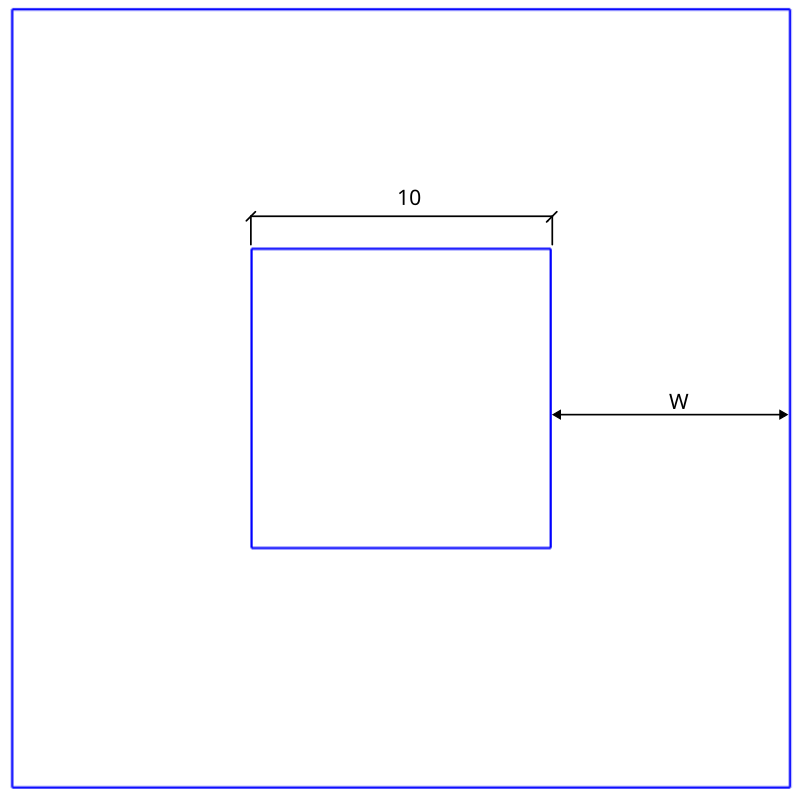
\includegraphics[width=0.3\linewidth]{sqwasher}
    \caption{The figure shows the geometry of the test washer in GMSH. All dimension are in $\mu m$}
    \label{fig:sqwasher}
\end{figure}

\subsection{Results}
Figure \ref{fig:steveComp} shows the results obtained by running the test setup. 
\begin{figure}[H]

    \centering
    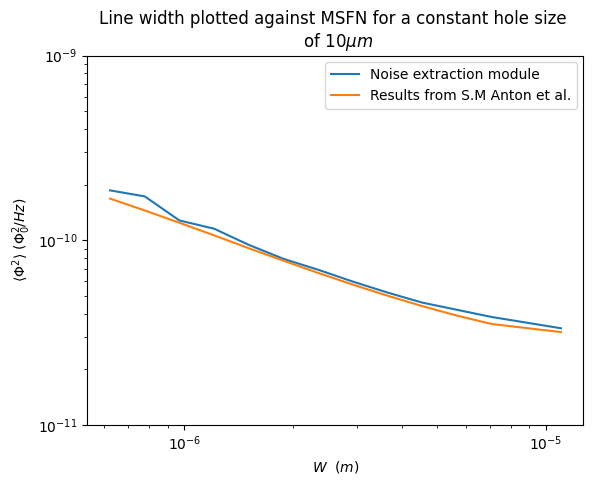
\includegraphics[width=0.4\linewidth]{steveComp}
    \caption{The plot shows the MSFN figure calculated by the noise extraction module as well as the figure calculated using \cite{msfnCode}}
    \label{fig:steveComp}
\end{figure}
From figure \ref{fig:steveComp} it is clear to see that the noise extraction module produces values in agreement with those obtained by S.M. Anton \textit{et al.} in \cite{fluxNoiseSquidsStevenAnton}. As shown in the previous section, the error decreases for an increase in optimisation iterations. One can therefore expect the noise extraction module to conform more closely to the results by S.M. Anton \textit{et al.} for a higher number of optimisation iterations. This could unfortunately not be tested due to memory limitations.

\section{Comparison with actual SQUID designs}
\subsection{Test setup}
The authors of \cite{fluxNoiseSquidsStevenAnton} performed accurate measurements of the PSD of a variety of SQUIDs. The authors also calculated the inferred MSFN by fitting each spectrum to equation \ref{eq:PSDfit}. Once the parameters in equation \ref{eq:PSDfit} where determined the authors calculated the MSFN figure. The authors measured MSFN values on 2 groups of SQUIDs. Both groups utilised Nb-AlOx-Nb junctions. The SQUIDs in group \textit{I} had film thickness of $150 nm$ and the SQUIDs in group \textit{II} had a film thickness of $200 nm$. 
\begin{equation}
    S_\Phi (f) = Af^{-\alpha}+C
    \label{eq:PSDfit}
\end{equation}
Both groups utilised the same square washer design but varied different parameters across each SQUID in the group. Group \textit{I} fixed the track width while varying the width of the washer. Group \textit{II} varied both the track width and the width of the washer. Table \ref{tab:sweepres} shows the results of the parameter sweep as well as the values of each parameter used in the sweep and figure \ref{fig:sqsweep} shows the square washer design along with what each parameter refers to.

\begin{figure}[H]
    \centering
    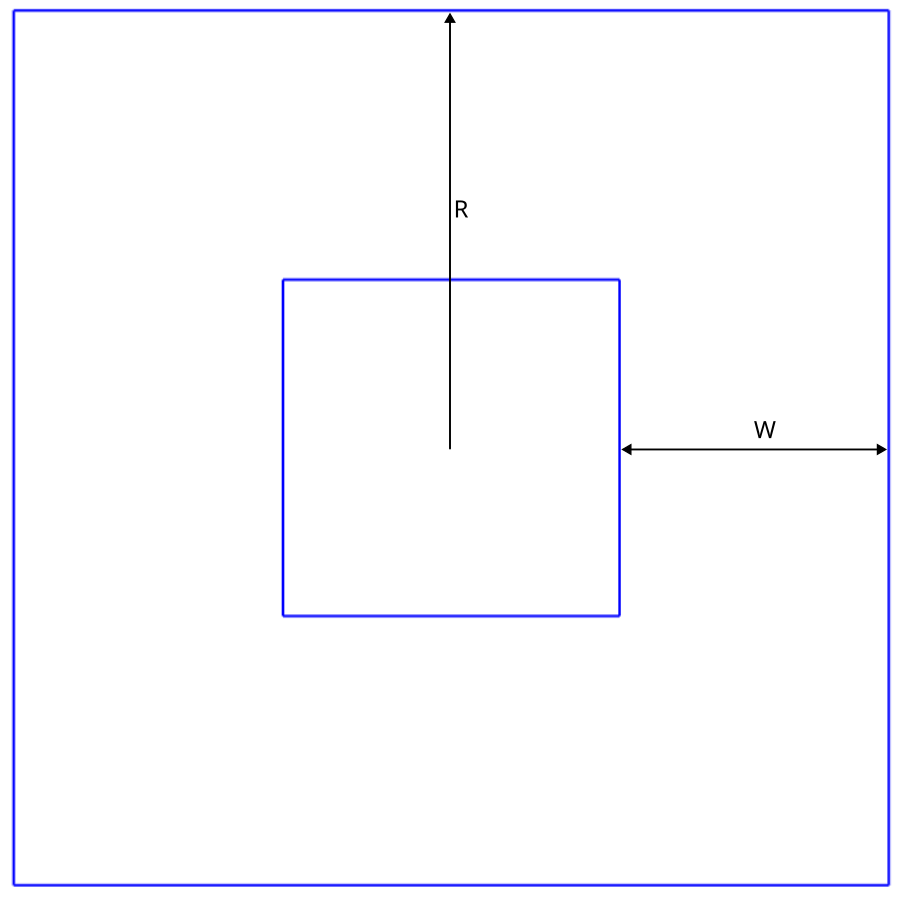
\includegraphics[width=0.4\linewidth]{sqsweep}
    \caption{A figure showing the parameters that are changed during the parameter sweep. W is referred to as the track width and R is referred to as the loop radius. 2R is the SQUID width.}
    \label{fig:sqsweep}
\end{figure}
\subsection{Results}
The MSFN figure cannot be measured directly. The power spectral density of the noise is measured. To relate the power spectral density to the mean square flux noise one can simply apply equation \ref{eq:PSDtoMSFN}.
\begin{equation}
    \langle \Phi^2 \rangle = \int_{f_1}^{f_2}S_\Phi (f) df
    \label{eq:PSDtoMSFN}
\end{equation} 
The limits of the integral are still the subject of debate \cite{fluxNoiseSquidsStevenAnton}. This is important to take note of as the choice of integration limits directly influence the result. The measured noise power in \cite{fluxNoiseSquidsStevenAnton} was calculated using $f_1 = 10^{-3}$ and $f_2 = 10^9$. Table \ref{tab:sweepres} shows the results of the parameter sweep. Figure \ref{fig:stevefig} is taken directly from \cite{fluxNoiseSquidsStevenAnton} and shows the flux noise measurements. For this comparison only the measurements at $0.1 K$ is used. 
\begin{table}[H]
    \centering   
    \begin{tabular}{lllll}
        \hline
        SQUID Number & R & W & MSFN (measured) ($\frac{\si{\nano}\Phi_0^2}{Hz}$) & MSFN (numerical) ($\frac{\si{\nano}\Phi_0^2}{Hz}$)\\ \hline
        I.1 & 12 & 0.5 & 4.5 & 111.924000 \\
        I.2 & 6 & 0.5 & 3 & 88.018600 \\
        I.3 & 3 & 0.5 & 1.2 & 0.121771 \\
        II.5 & 40 & 15 & 1 & 0.110498 \\
        II.1 & 265 & 240 & 2 & 0.098736 \\
        II.3 & 85 & 60 & 0.8 & 0.043155 \\ \hline
    \end{tabular}
    \caption{The table shows the measured MSFN figures from \cite{fluxNoiseSquidsStevenAnton} and the MSFN values calculated using the noise extraction module. The parameters R and W are listed in $\si{\micro m}$. The SQUID number uses the same numbering as used in \cite{fluxNoiseSquidsStevenAnton}. The table is sorted by the numerical MSFN figure in ascending order.}
    \label{tab:sweepres}
\end{table}

\begin{figure}[h]
    \centering
    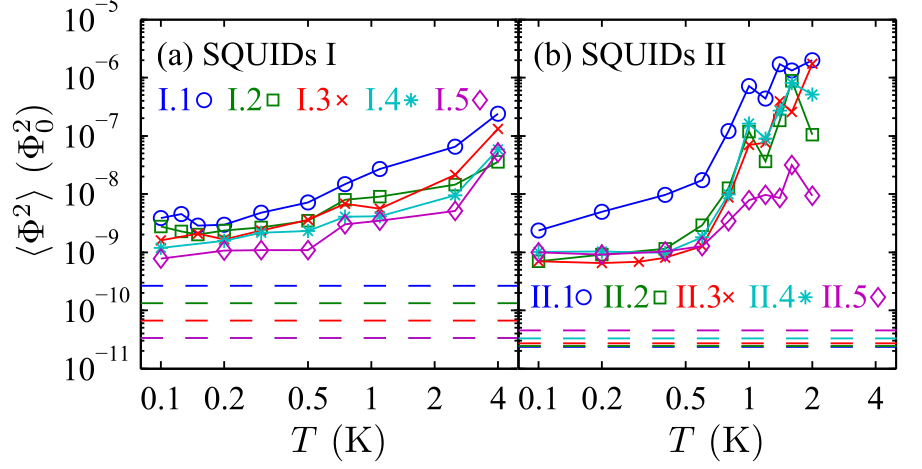
\includegraphics[width=0.5\linewidth]{stevenfig}
    \caption{The figure shows the various flux noise measurements taken in \cite{fluxNoiseSquidsStevenAnton}. The dashed line is predicted flux noise from the analytic equation \ref{eq:ThinFilmMSFN}.}
    \label{fig:stevefig}
\end{figure}

Table \ref{tab:sweepres} demonstrates that there is a large discrepancy between the measured MSFN figures and the figures calculated using the noise extraction module. If we only consider SQUIDs in group \textit{I} for the moment, we observe that the noise extraction module calculates MSFN figures that follow the same trend as the measured values. The SQUID with the largest measured MSFN value is also the SQUID with the largest MSFN figure calculated by the noise extraction module. If we consider only the SQUIDs in group \textit{II} then this trend is violated. We do note that in group 2 the analytical predictions roughly follow the same trend. The authors noted that a potential source of error in the inferred MSFN figures is the sensitivity of the alpha parameter. Fitting the measured PSD to equation \ref{eq:PSDfit} will lead to some error. The authors noted that at low temperatures a $0.03$ change in $\alpha$ can change the inferred MSFN figure by a factor of $1.6$. The violation of the trend in group \textit{II} can easily be accounted for by error in the $\alpha$ parameter. The authors also noted their difficulty in reconciling their data with the uncorrelated surface spin model and suggested that their data is consistent with a model where there is strong correlation between individual spins \cite{fluxNoiseSquidsStevenAnton}. \par
In this context one could make the argument that the module is useful for design as it can enable designers to compare designs but not useful for accurately predicting MSFN figures. More data over a wider range is required to conclusively make this claim as errors in fitting the data makes it hard to compare designs with similar MSFN figures.

\graphicspath{{conclusion/fig/}}

\chapter{Summary and Conclusion}
\label{chap:conclusion}

In chapter \ref{chap:litreview} the basic theory and applications of superconductors were discussed. Once a suitable understanding of the DC SQUID was established an understanding of the importance that low-frequency noise has on the performance of a SQUID was emphasized. It was noted that in fields such as geophysics and biomagnetism the low frequency noise performance of a SQUID is critical. It was also noted that in the Josephson phase qubit, low-frequency noise is the primary cause of decoherence. Literature on previous attempts to model this noise was reviewed, and it was clear that it is generally agreed that the noise is a result of the random reversal of electronic spins on the surface of the SQUID washer. The previous attempts at numerically and analytically calculating the low-frequency noise power were reviewed. Through this review, the work of S. M. Anton \textit{et al.} was identified as the best fit for the objectives of this project. The work laid out a numerical framework for the calculation of the MSFN figure that is flexible and robust. \par
Chapter \ref{chap:solutiondevelopment} started by refining the problem and clarifying the objectives of the project. It determined that the development of 2 different modules (the noise extraction and mesh optimisation modules) where necessary. The chapter continued by developing the high level system design. It gave the necessary context to understand where the noise extraction and mesh optimisation modules would work in the system. The next section described the detailed design of each module. It starts with the simplest module: the mesh optimisation module. The optimisation required the limiting of either the change in the magnetic flux density or the change in current density across mesh elements. The current density was ultimately chosen. The chapter further described how the mesh optimisation module systematically subdivides the lines joining nodes in the mesh to ensure that the current density does not change more than specified between adjacent nodes. The next section described the design of the noise extraction module. This section described the challenge of finding a suitable method for integrating over the surface of the SQUID. It was decided that the best option was to partition the mesh into regions defined by the Voronoi tessellation of the nodes. It was then shown how the Voronoi tessellation can be found from the triangular mesh. The algorithm for calculating the area of each Voronoi cell is described and the workaround necessary to ensure the points in the Voronoi cells are ordered is stated. 
\par
Chapter \ref{chap:results} described the general testing methodology before describing how each module is tested. The noise extraction module was first tested on an unoptimized mesh, and it was found that the module produced values in accordance with the analytic predictions. It was then concluded that the noise extraction module worked as expected. The mesh optimisation module was tested to answer three questions: How many iterations are required? Does the optimized mesh provide accurate results? Is the optimisation process faster than just performing the analysis with a very fine mesh from the start? It was found the optimal number of iterations is between 1 and 2. It was noted that the choice ultimately comes down to how accurate the user wants to be. The testing also revealed that the optimized mesh after 2 iterations produced accurate results in substantially shorter times compared to simply using a finely meshed structure. The chapter continues by testing the full system against the measured and numerical results of S. M. Anton \textit{et al}. The noise extraction showed good correspondence with the numerical results but large discrepancies were observed between the numerical results and measured results. It was concluded that the discrepancy is large enough to invalidate the use of the system for precisely predicting MSFN values. The trend seen across the test SQUIDs revealed that the system could be used to compare designs but more data on SQUIDs with larger variations in MSFN figures is necessary to make any conclusive claim about this.
\par
It can be concluded that the extensive testing and validation of the system verifies that it is working as expected. That is, it provides MSFN figures consistent with those predicted by the uncorrelated surface spin model. This alludes to a possible inaccuracy in the theory. As noted in \cite{fluxNoiseSquidsStevenAnton} it is possible that the spins are not uncorrelated but instead form uncorrelated clusters of correlated spins. This project lays the groundwork for further investigation of the surface spin model as it implements a flexible implementation that is valid for any geometry. Further investigation includes the collection of more data over a wider range of SQUID loop geometries but also the modification of the noise extraction module to model clusters of correlated spins. The authors of \cite{fluxNoiseSquidsStevenAnton} point out that is not known whether spins are confined spatially or move across the surface such as in the spin diffusion model. \par 
The hope is that the implementation presented in this project can serve as a foundation for better models. Recent studies suggest that the spin diffusion model could explain the experimental observations \cite{FNdisord,FNtempdepend}. Both studies utilise the same principle of reciprocity to calculate the contribution of individual spins to the flux noise implemented in this project. As noted in \cite{fluxNoiseSquidsStevenAnton} the modification only changes how each spin contribution is summed. As such, the natural next step is to investigate how spin clusters form and develop a methodology for determining a suitable weighting function to model the contribution of spin-spin interactions. 

% Bibliography
\bibliography{mybib}

% End matter
\appendix
\graphicspath{{appendices/}}

\chapter{Example settings file}
\makeatletter\@mkboth{}{Appendix}\makeatother
\label{appen:settings}
\begin{figure}[H]
    \centering
    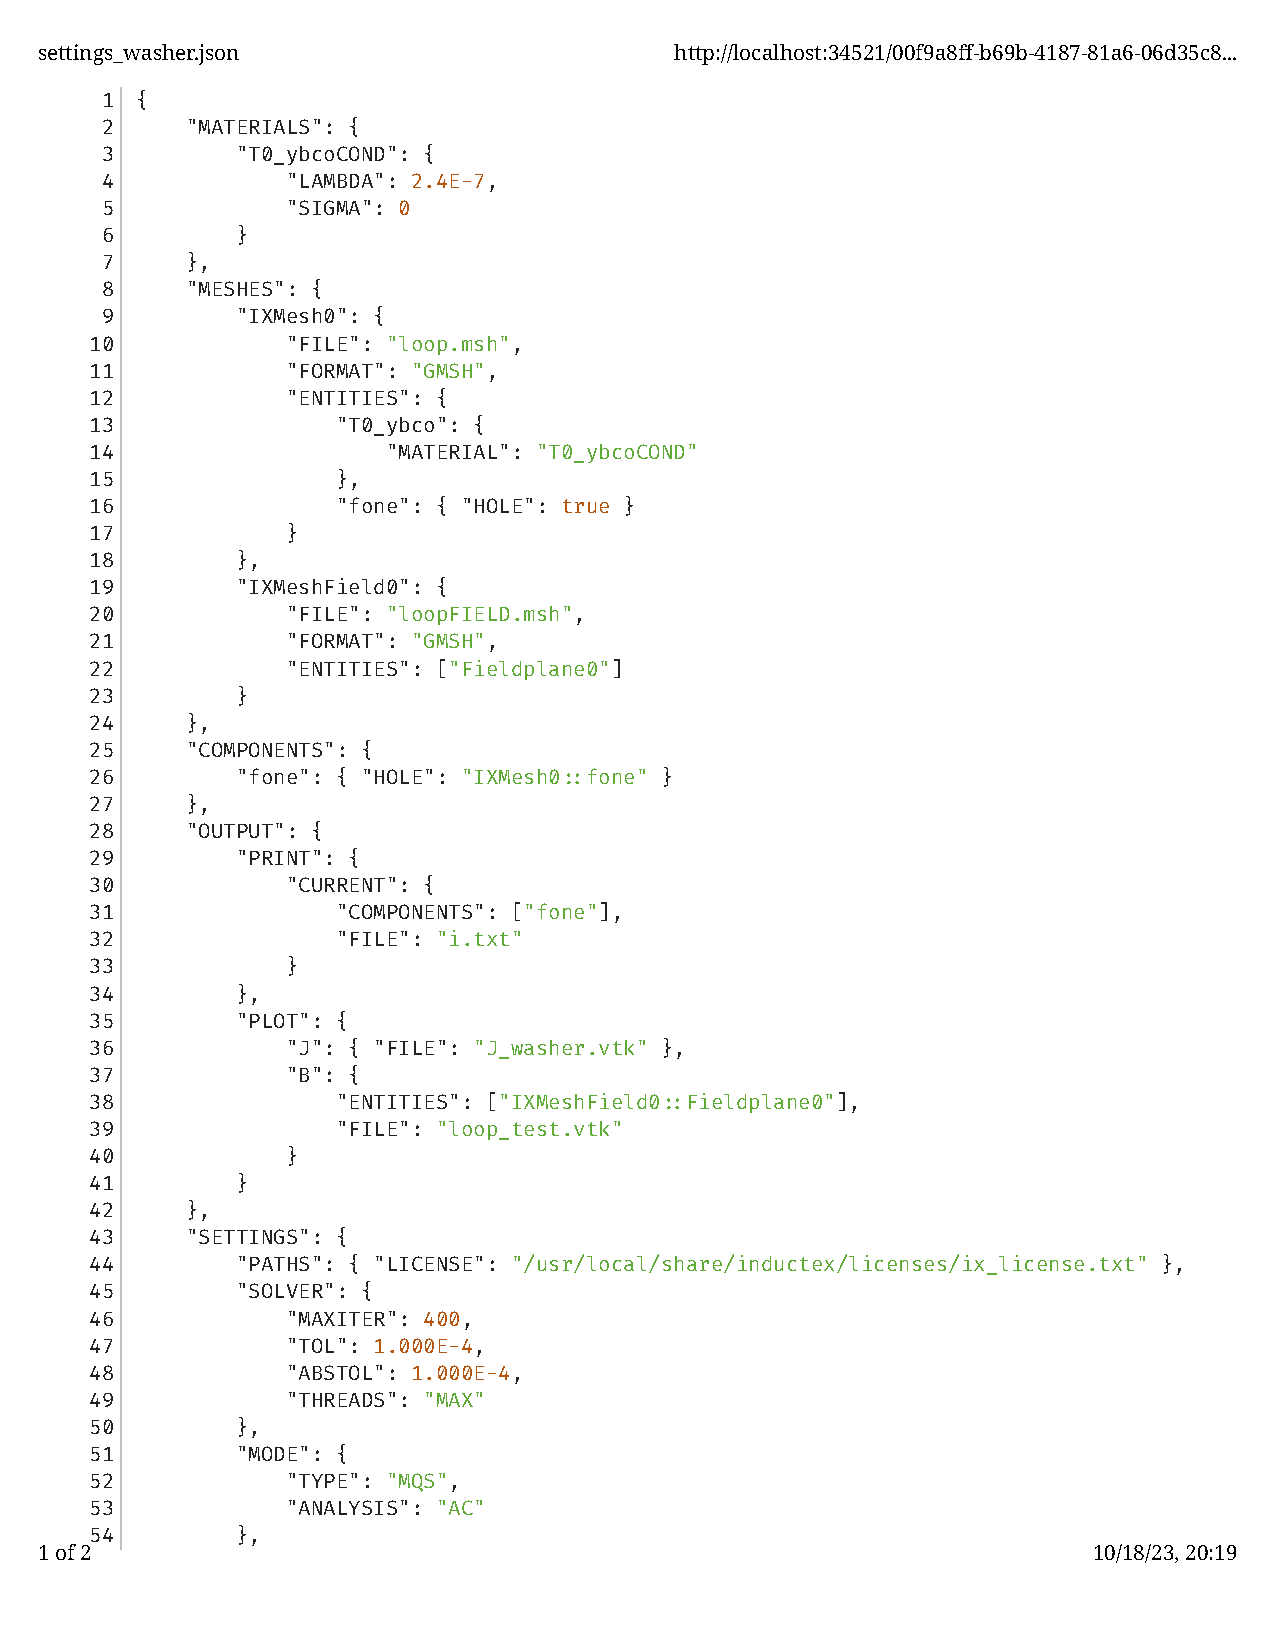
\includegraphics[width=0.9\textwidth]{settings.pdf}
    \label{fig:sett1}
\end{figure}
\newpage
\begin{figure}[H]
    \centering
    \includegraphics[width=0.9\textwidth,page=2]{settings.pdf}
    \label{fig:sett2}
\end{figure}

\chapter{Project Planning Schedule}
\makeatletter\@mkboth{}{Appendix}\makeatother
\label{appen:PPS}

\begin{table}[H]
    \centering
    \begin{tabular}{lll}
        \hline
        \textbf{Task Name}                                   & \textbf{Start Date} & \textbf{Due Date} \\ \hline
        Skripsie Admin                                       & 06/28/2023          & 06/30/2023        \\
        Read Feynmann lectures volume III                    & 07/01/2023          & 07/20/2023        \\
        Read S.M. Anton's PhD thesis                         & 07/21/2023          & 08/07/2023        \\
        Complete and submit GA plan                           & 08/08/2023          & 08/09/2023        \\
        Develop, Implement and test noise extraction module  & 08/10/2023          & 09/03/2023        \\
        Develop, Implement and test mesh optimisation module & 09/04/2023          & 09/23/2023        \\
        Determine Lit review topics                          & 08/10/2023          & 08/12/2023        \\
        Write first 3 sections of lit review                 & 08/13/2023          & 09/02/2023        \\
        write the last three sections of lit review              & 09/03/2023          & 09/23/2023        \\
        write design section                                 & 09/24/2023          & 10/07/2023        \\
        obtain results for results section                   & 09/24/2023          & 10/11/2023        \\
        write results section                                & 10/12/2023          & 10/22/2023        \\
        write introduction                                   & 10/18/2023          & 10/20/2023        \\
        submit preliminary report                            & 10/21/2023          & 10/21/2023        \\
        Make changes to report as recommended by supervisor  & 10/23/2023          & 10/29/2023        \\
        Spelling and grammar checks                          & 10/31/2023          & 10/31/2023        \\
        Write abstract                                       & 10/30/2023          & 10/30/2023        \\
        Create poster and video                              & 11/01/2023          & 11/04/2023        \\
        final check and submission                           & 11/05/2023          & 11/05/2023        \\
        final submission due                                 & 11/05/2023          & 11/06/2023        \\ \hline
        \end{tabular}
        \caption{The project planning schedule}
        \label{tab:pps}
    \end{table}


\chapter{Outcomes Compliance}
\makeatletter\@mkboth{}{Appendix}\makeatother
\label{appen:OC}

\section{GA 1. Problem Solving}
This project required the implementation of an algorithm to calculate the expected noise power in a SQUID. It extends on previous works by generalizing existing techniques to work on any geometry. The algorithm converts a complex 3-dimensional mesh into a single number. The task does not have a defined solution and requires solving many individual problems including but not limited to numerically calculating a surface integral, electromagnetic simulation with TetraHenry, mesh optimisation and modelling of superconducting structures. The details of these challenges are discussed in Chapter \ref{chap:nex} and \ref{chap:meshopt}.

\section{GA 2. Application of Scientific and Engineering Knowledge}
The topic relied on a good understanding of scientific and engineering concepts introduced in my undergraduate years as well as the application of this knowledge to solve open-ended problems. It required knowledge of calculus, vector calculus, electromagnetism, and programming. Along with topics introduced in the undergraduate years, a rudimentary understanding of quantum mechanics and superconductors was needed. Chapters \ref{chap:litreview} and \ref{chap:solutiondevelopment} show the fulfilment of these outcomes.
\section{GA 3. Engineering Design}
The problem statement was very open-ended and required refinement (Chapter \ref{chap:dgoals}). System design techniques were used to solve the engineering design problem in Chapter \ref{chap:high level design}. Once the problem was formally defined it was broken down into smaller sub-problems in Chapter \ref{chap:ddesign}. Solving the sub-problems required drawing knowledge from a wide variety of sources about the topics listed in GA 2.
\section{GA 4. Investigations, experiments and data analysis}
Once the system was implemented an investigation was performed to determine the validity of the results. This required using previous results obtained by simulation as well as physical tests and comparing them to results obtained from my system. The system was tested for accuracy (how closely the output of my system when operating on a previously solved problem matches the true solution) and performance. The testing procedure was designed and then implemented using Python. The regex and OS modules were used to perform parameter sweeps and automate testing. The data output from this testing procedure was analysed to extract conclusions about the performance and accuracy of the system. This achievement of this outcome is demonstrated in Chapter \ref{chap:results}. 
\section{GA 5. Engineering methods, skills and tools, including Information Technology}
To perform the data analysis required as mentioned in GA 4 jupyter notebooks were used in conjunction with the numpy, pandas, matlpotlib and seaborn libraries. The results of this analysis are shown in \ref{chap:results}. Electromagnetic simulations were done with TetraHenry and InductEx. CMake and VCPKG were used to manage compilation and code dependencies. Knowledge of the CLion IDE was crucial to the implementation of this project. GitHub and Git were used for project backup and source control. To model the 3D SQUID structures they had to be created with GMSH. This was done using the GMSH scripting language. Evidence of the above can be found in the GitHub repository \cite{paulcode}. ParaView was used to quickly visualise the results generated by TetraHenry. To improve personal productivity Trello was used to track active tasks as well as future tasks.

\section{GA 6. Professional and technical communication}
The project includes a written report and an oral presentation. These demonstrate competence to communicate effectively, both orally and in writing. Communication with my supervisor included progress reports both as presentations and demonstrations of work progress.

\section{GA 8. Individual work}
I was solely responsible for the completion of my project with little to no input from others. 

\section{GA 9. Independent Learning Ability}
The project required an understanding of complex topics not previously encountered by me. The broad topic gave no context to the required knowledge for the successful completion of the project. Chapter \ref{chap:litreview} demonstrates the process through which I acquired the necessary knowledge. It explores the topics needed to grasp the problem in the order by which they were encountered by me.  

\end{document}

